%appendixprefix sorgt daf�r, dass "Anhang" vor jedem Anhang steht
%openany sorgt daf�r, dass ein Kapitel auf jeder Seite beginnen kann
%        nicht nur rechts
%bibtotoc sorgt daf�r, dass das Literaturverzeichnis automatisch im
%         Inhaltsverzeichnis erscheint
\documentclass[fontsize=11pt,paper=a4,parskip=half,draft=false,appendixprefix,bibtotoc]{scrartcl}
% uncomment the following line (mutual exclusive to the one above) to enter the draft mode.

\usepackage{ifthen}
\newboolean{public}
\setboolean{public}{false}

% For screen viewing it is nice to have references marked in a slightly different
% color than the rest of the text. Since they will be hyperlinks to the 
% referenced objects.
%\usepackage[pdftex,
%             pdftitle={},
%             colorlinks,
%             linkcolor={titleblue},
%             citecolor={mygrey},
%             urlcolor={black},
%             plainpages={false},
%             bookmarksnumbered={true},
%             pdfauthor={},
%             pdfsubject={},
%             pdfkeywords={},
%             pdfstartview={}]{hyperref}
             
             %was:
             %pdfstartview={FitBH}]{hyperref}

% For the final printouts (remember - you need at least three - one for each examiner and one for the archive 
% [ This might have changed - so contact the "Pr�fungsamt" about the current regulations !! ] - it is better
% to have all text in the same color (namely black).
% 
\usepackage[pdftex,
            pdftitle={},
            colorlinks,
            linkcolor={black},
            citecolor={black},
            urlcolor={black},
            plainpages={false},
            bookmarksnumbered={true},
            pdfauthor={},
            pdfsubject={},
            pdfkeywords={},
            pdfstartview={}]{hyperref}
\pdfcompresslevel=9

\pdfoutput=1
%\tracingstats=2
%\usepackage{layout}
% german language support (hyphenation etc)  
%\usepackage{ngerman}

% support for latin1 characters. That means you can enter � � � � directly
% no need for "a "u "� "s anymore
\usepackage[latin1]{inputenc}
 
% provides the \url{} command to pretty print urls
\usepackage{url}

% needed for a german bibliography-style (s. below)
%\usepackage{bibgerm}
%\usepackage{babelbib}
%\selectbiblanguage{ngerman}

%\usepackage[comma,numbers,sort&compress,nonamebreak]{natbib}
%\usepackage{bibgerm}
\bibliographystyle{alphadin}

% allows text flowing around figures.
\usepackage{wrapfig}

% allows to \includegraphics
\usepackage{graphicx}

% defines some standard colornames like "black" etc.
\usepackage{color}

% allows to color tablecells
\usepackage{colortbl}

% provides an easier interface to if-then-else constructs in 
% custom macros
\usepackage{ifthen}

% allows tables to break over pages.
\usepackage{supertabular}

% allows to have different kinds paper orientations in the same pdf-documnent
\usepackage{pdflscape}

% allows to specify absolute texpos for textboxes. This is generally only important for the titlepage
\usepackage[absolute]{textpos}

% allows to enumerate different figures with a) b) in the same figure-environment.
\usepackage{subfigure}

% introduces new commands for more beautiful tables
\usepackage{booktabs}
\usepackage{multirow}

% source code listings
\usepackage{listings}

\lstset{
	basicstyle=\small\ttfamily,
%	keywordstyle=\bfseries % typewriter font has no bold counterpart
	captionpos=b,
	float=htbp,
	frame=tlrb
}
\renewcommand*\lstlistingname{Textauszug}
\renewcommand*\lstlistlistingname{Textauszugsverzeichnis}

% allows \Checkmark and more
\usepackage{bbding}

% finetune the gaps between figure and text in the subfigure environment (basically close the gap as much as possible)
\renewcommand{\subfigtopskip}{0pt}
\renewcommand{\subfigbottomskip}{0pt}

% some color definitions for the pdf statements below
\definecolor{mygrey}{rgb}{0.45,0.45,0.45}
\definecolor{mydarkgrey}{rgb}{0.2,0.2,0.2}
\definecolor{red}{rgb}{1.0,0.33,0.33}
\definecolor{orange}{rgb}{1.00,0.73,0.33}
\definecolor{yellow}{rgb}{0.95,0.92,0.}
\definecolor{lightgreen}{rgb}{0.3,0.95,0.46}
\definecolor{titleblue}{rgb}{0.03,0.10,0.46}

\usepackage[latin1]{inputenc}
\usepackage[toc]{glossaries}
\makeglossaries
\renewcommand{\glossaryname}{Glossar}

\newglossaryentry{AES}{name=AES, description={Advanced Encryption Standard, auch Rijndael-Algorithmus; symmetrischer Blockchiffre \cite{rijndael}}}

\newglossaryentry{ASCII}{name=ASCII, description={American Standard Code for Information Interchange; Zeichensatz mit 7-Bit-Kodierung}}

\newglossaryentry{Base64}{name=Base64, description={Kodierung, die 8-Bit Bin�rdaten auf eine 6-Bit gro�e Zeichenmenge abbildet}}

\newglossaryentry{Brute-Force-Angriff}{name=Brute-Force-Angriff, description={Sicherheitsangriff auf ein Kryptosystem durch das Ausprobieren aller m�glichen L�sungen. In der Theorie immer erfolgreich, in der Praxis meist aufgrund eines zu gro�en L�sungsraums nicht in einem akzeptablen Zeitraum durchf�hrbar}}

\newglossaryentry{CFB-Modus}{name=CFB-Modus, description={Cipher Feedback Mode; Betriebsmodus f�r Blockchiffre, siehe Kapitel \ref{cfb}}}

\newglossaryentry{Denial-of-Service-Angriff}{name=Denial-of-Service-Angriff, description={Angriff auf die Verf�gbarkeit eines Systems, h�ufig durch �berlastung eines Dienstes}}

\newglossaryentry{Firewall}{name=Firewall, description={technisches Sicherheitskonzept zum Schutz von Rechnernetzen und deren \glslink{Host}{Hosts}}}

\newglossaryentry{Handshake}{name=Handshake, description={Er�ffnung einer Sitzung in einem Kommunikationsprotokoll}}

\newglossaryentry{Hash-Algorithmus}{name={Hash-Algorithmus}, plural={Hash-Algorithmen}, description={bildet Eingabedaten eindeutig auf einen Ausgabewert (Hash-Wert) ab. Der Hash-Wert eines kryptographisch sicheren Algorithmus erm�glicht keine R�ckschl�sse auf die Eingabedaten}}

\newglossaryentry{HMAC}{name=HMAC, description={Keyed-Hash Message Authentication Code, siehe Kapitel \ref{hmac}}}

\newglossaryentry{Host}{name=Host, plural=Hosts, description={Netzkomponente, die dem Rechnernetz Dienste zur Verf�gung stellt}}

\newglossaryentry{HTTP}{name=HTTP, description={Hypertext Transfer Protocol; Daten�bertragungsprotokoll}}

\newglossaryentry{HTTP-Proxy}{name=HTTP-Proxy, description={Netzkomponente, die \gls{HTTP}-Verbindungen vermittelt}}

\newglossaryentry{HTTPS}{name=HTTPS, description={HTTP �ber \gls{SSL/TLS}}}

\newglossaryentry{IP}{name=IP, description={Internet Protocol; Netzwerkprotokoll auf Vermittlungsschicht des \glslink{OSI-Modell}{OSI-Modells}}}

\newglossaryentry{IP-Spoofing}{name=IP-Spoofing, description={Versenden von \gls{IP}-Paketen mit gef�lschter Quelladresse zur Vort�uschung einer fremden Identit�t}}

\newglossaryentry{Java SE}{name=Java SE, description={Java Platform, Standard Edition; Java-Laufzeitumgebung f�r Desktop- und Serversysteme}}

\newglossaryentry{kerckhoff}{name={Kerckhoffs' Prinzip}, description={Kryptographisches Prinzip von Auguste Kerckhoffs (1835--1903), nach dem die Sicherheit eines Kryptosystems durch die Geheimhaltung des Schl�s\-sels und nicht der Geheimhaltung des Algorithmus hergestellt wird}}

\newglossaryentry{Media Type}{name={Media Type}, description={auch MIME Type; Klassifizierungsschema f�r Datenformate \cite{rfc2046}}}

\newglossaryentry{MITM-Angriff}{name=Man-in-the-Middle-Angriff, description={Sicherheitsangriff auf eine Daten�bertragung, bei dem sich ein An\-grei\-fer zwischen den Kommunikationsteilnehmern befindet und deren �bertragung abh�ren und manipulieren kann}}

\newglossaryentry{OSI-Modell}{name=OSI-Modell, description={siebenschichtiges Referenzmodell zum Entwurf von Kommunikationsprotokollen}}

\newglossaryentry{Padding}{name=Padding, description={Auff�llen von Nutzdaten mit inhaltslosen Bytes, um eine Datenstruktur vorgegebener Gr��e einzuhalten}}

\newglossaryentry{PMS}{name=PMS, description={Property Management System; Anwendung zur elektronischen Verwaltung und Abrechnung im Hotelgewerbe}}

\newglossaryentry{Polling}{name=Polling, description={zyklisches Abfragen eines Zustands}}

\newglossaryentry{POSIX}{name=POSIX, description={Portable Operating System Interface; standardisierte Betriebssystemschnittstelle f�r Anwendungen, insbesondere im Unix-Bereich g�ngig}}

\newglossaryentry{Replay-Angriff}{name={Replay-Angriff}, plural={Replay-Angriffe}, description={Sicherheitsangriff durch Wiedereinspielung zuvor aufgezeichneter Daten}}

\newglossaryentry{RFID}{name=RFID, description=Radio Frequency Identification; elektronisches Identifizierungsverfahren}

\newglossaryentry{Router}{name=Router, description={vermittelnde Komponente in einem Rechnernetz}}

\newglossaryentry{RS-232}{name=RS-232, description=eigentlich EIA/TIA-232; serielle Schnittstelle zum Anschluss von Peripherieger�ten}

\newglossaryentry{Seitenkanalangriff}{name=Seitenkanalangriff, plural=Seitenkanalangriffe, description={Sicherheitsangriff auf eine bestimmte Implementation eines kryptographischen Verfahrens durch Beobachtung externer Parameter, etwa der verbrauchten Rechenzeit oder der Speichernutzung}}

\newglossaryentry{SHA}{name=SHA, description={Secure Hash Algorithm; eine Familie von kryptographischen \glslink{Hash-Algorithmus}{Hash-Al\-go\-rith\-men} mit Ausgabegr��en von 160 bis 512 Bit}}

\newglossaryentry{Sniffing}{name=Sniffing, description={Abh�ren des Datenverkehrs im lokalen Netzwerk}}

\newglossaryentry{SSL/TLS}{name={SSL/TLS}, description={Secure Sockets Layer/Transport Layer Security; Kommunikationsprotokoll zur kryptographisch sicheren Daten�bertragung}}

\newglossaryentry{Stateful Packet Inspection}{name={Stateful Packet Inspection}, description={Mechanismus bei \glslink{Firewall}{Firewalls}, um jedes einzelne Datenpaket einer zustandsbehafteten Sitzung zuzuordnen}}

\newglossaryentry{StAX}{name=StAX, description={Streaming API for XML; Programmierschnittstelle zur strombasierten Verarbeitung von XML-Daten}}

\newglossaryentry{TCP}{name=TCP, description={Transmission Control Protocol; Netzwerkprotokoll auf Transportschicht des \glslink{OSI-Modell}{OSI-Modells} \cite{rfc793}}}

\newglossaryentry{USB}{name=USB, description=Universal Serial Bus; serielles Bussystem zum Anschluss von Peripherieger�ten}

\newglossaryentry{UML}{name=UML, description={Unified Modeling Language; grafische Notation zur Systemmodellierung}}

\newglossaryentry{Unixzeit}{name=Unixzeit, description=gel�ufiges Format zur Angabe eines Zeitpunkts: Anzahl Sekunden seit dem 1. Januar 1970 00:00:00 UTC}

\newglossaryentry{URL}{name=URL, description={Uniform Resource Locator; Klassifizierungsschema f�r Ressourcen in einem Rechnernetz \cite{rfc3986}}}

\newglossaryentry{UTF-8}{name=UTF-8, description={8 Bit Unicode Transformation Format; ein Kodierungsformat des Unicode-Zei"-chen"-satzes}}

\newglossaryentry{XMPP}{name=XMPP, description={Extensible Messaging and Presence Protocol; Netzwerkprotokoll, insbesondere f�r Instant Messaging \cite{rfc3920}}}

\newglossaryentry{XML}{name=XML, description={Extensible Markup Language; textbasierte Auszeichnungssprache zur Speicherung und zum Austausch von Daten}}


% some configuration for the amount of text on a single page
\usepackage{typearea}\areaset[1.5cm]{418pt}{658pt}
\setlength{\headheight}{37pt}

% To avoid nasty mistakes like having comments directly in the textflow
% the following \todo macro was defined. With that you can enter
% \todo{What I still have to do here} 
% inside of your text and a marker will appear at the page's margin with the 
% text "What I still have to do here".
% The first line activates this feature. If you comment it out and uncomment
% the second line below there will be no error messages and no todos will be shown
% anymore. So - even if you have forgotten to delete one of them - they will not appear
% in the final printout. 
\newcommand{\todo}[1]{\marginpar{\textcolor{red}{ToDo:} #1}}
%\newcommand{\todo}[1]{}

% We recommend to split your document into several files. Usually one for every chapter is a 
% good idea. If you follow this guideline (how to assemble these files in a single document
% see two paragraphs below) you will be able to single out chapters via the \includeonly{}
% command. Using this mechanism page numbering and references of the full run before will be
% preserved. This also nice, if your latex run tends to get slow and you need to fine tune 
% some formatting in one chapter - just include that one. The rest (or at least the ones before
% the one currently under construction) will remain untouched. This means a boost in compilation time.
%\includeonly{chapter2}

\usepackage{tikz}

\usetikzlibrary{shapes.geometric}
\usetikzlibrary{calc}
\usetikzlibrary{fit}
\usetikzlibrary{backgrounds}
\usetikzlibrary{positioning}
\usetikzlibrary{arrows}
\usetikzlibrary{decorations.pathreplacing}
\usetikzlibrary{shapes.misc}

% ---------------------------------------------------------------------------- %
% Tikz definitions

\tikzset{port/.style={shape=circle,inner sep=0,draw=black,fill=white,minimum height=2pt,minimum width=2.5pt}}
\tikzset{point/.style={shape=circle,inner sep=0,fill=black,minimum height=1pt,minimum width=1pt}}
%\tikzset{gnode/.style={shape=circle,inner sep=0,fill=black,minimum height=.1cm,minimum width=.1cm}}
\tikzset{hyperedge/.style={shape=rectangle,draw,inner sep=0,minimum width=.4cm,minimum height=.4cm}}
\tikzset{marr/.style={shorten <=2pt,shorten >=2pt,->}}
%\tikzset{nodelabel/.style={minimum height=.4cm,font=\scriptsize}}
\tikzset{edgelabel/.style={circle,inner sep=1pt}}
\tikzset{cross/.style={cross out, draw=black, minimum size=2*(#1-\pgflinewidth), inner sep=0pt, outer sep=0pt},cross/.default={1pt}}

\tikzset{gnode/.style={shape=circle,fill=black,inner sep=0mm,minimum size=2mm}}
\tikzset{glab/.style={inner sep=1pt,font=\scriptsize}}

\tikzset{every fit/.style={shape=rectangle,inner sep=5pt}}

\tikzset{
	mono/.style={>->},
	%	gnode/.style={circle,fill=black,inner sep=0mm,minimum size=2mm,font=\scriptsize,text=white},
	gedge/.style={->,>=latex},
	arlab/.style={inner sep=1pt,font=\scriptsize},
	%	glab/.style={inner sep=1pt,font=\scriptsize},
	hyperedge/.style={shape=rectangle,draw,inner sep=0,minimum width=1cm,minimum height=.4cm},
	point/.style={shape=circle,inner sep=0,fill=black,minimum height=1pt,minimum width=1pt}
}

\newcommand\graphboxthick[2][grbox]{
	\begin{pgfonlayer}{background}
		\node[fit=#2] (#1) {};
		\fill[black!20,rounded corners=2mm,postaction={draw,black}] (#1.north west) -- (#1.north east) -- (#1.south east) -- (#1.south west) -- cycle;
	\end{pgfonlayer}
}

\newcommand\substx[2]{
	($ (0,0)!#1!(0,1) + (#2,0) $)
}

\newcommand\substy[2]{
	($ (0,0)!#1!(1,0) + (0,#2) $)
}

\usepackage{mathtools}

\usepackage[titletoc,title]{appendix}

\usepackage{wasysym}
\usepackage{amssymb}

\begin{document}
% the next two lines influence the detailedness of the table of contents
% and to what structure depth numbers are written before sections/subsections/paragraphs
% You should not touch this
\setcounter{tocdepth}{3}
\setcounter{secnumdepth}{3}

% here the titlepage is included. Look into the file "titelseite.tex" to 
% adapt it to your needs (name, title etc.)
% Titelseite braucht folgenden  Eintrag
% \usepackage[absolute]{textpos}
% textpos ist nicht Bestandteil von tetex
% kann aber von dante heruntergeladen werden
\begin{titlepage}
\vspace*{-1cm}
\newlength{\links}
\setlength{\links}{0.9cm}
\setlength{\TPHorizModule}{1cm}
\setlength{\TPVertModule}{1cm}
\textblockorigin{0pt}{0pt}

\sf
\LARGE

\begin{textblock}{16.5}(2.8,2.6)
 \hspace*{-0.25cm} \textbf{UNIVERSIT�T DUISBURG-ESSEN} \\
 \hspace*{-1.15cm} \rule{5mm}{5mm} \hspace*{0.05cm} FAKULT�T F�R INGENIEURWISSENSCHAFTEN\\
 \large{}ABTEILUNG INFORMATIK UND ANGEWANDTE KOGNITIONSWISSENSCHAFT \\
\end{textblock}


%Hier Titel, Name, und Matrikelnummer eintragen, \\ make a newline
\begin{textblock}{14.5}(3.2,8.5)
	\large
	{ \bf Master's Thesis} \\[1cm]
	{\LARGE \Large\bf Infinite Games: Algorithms and Reductions} \\[1.3cm]
	Maxime Nederkorn\\
	Matrikelnummer: 3004376
\end{textblock}


\begin{textblock}{7}(13.5,17.5)
%\begin{textblock}{10}(10.5,17.5)
\includegraphics[scale=1.0]{unilogo.pdf}\\
\normalsize
\raggedleft
%Seminarausarbeitung an der\\
Department of Computer Science and Applied Cognitive Science \\
Faculty of Engineering \\
University of Duisburg-Essen \\[2ex]

31. January 2022\\[15ex]
\raggedright
% Supervisors
{\bf Examiners:} \\
Prof. Dr. Barbara K�nig\\
Prof. Dr. Janis Voigtl�nder\\[1em]
{\bf Advisor:} \\
Richard Eggert
\end{textblock}

%\begin{textblock}{16.5}(3.2,15)
%\ifthenelse{\boolean{public}}{\textsl{�ffentliche Version}}{}
%\end{textblock}

\end{titlepage}

\tableofcontents
%\listoffigures
%\listoftables
%\lstlistoflistings

% To assemble the whole document
% Please be aware that each file will begin on a new page
% therefore chapters should be put into such a file.
% There cannot be an include statement inside of an "included" file.
% So if you want to further divide your document - use \input inside of 
% the included files. \input will not begin on a new page.
\section{Introduction}
There are practical applications (cite) which are able to be modeled by or reduced to various games. Considering the many ways there are to solve those games, the possibility to (repeatedly) reduce them to one another and various ways to implement any of those algorithms there are many potential means to solve problems on those games. We want to see how the different ways to solve problems, the reductions between those problems and the combination of the two play out and compare to one another in a real-world implementation.
\subsection{Task}
The games we concern ourselves here are \textit{Parity Games} (PG), \textit{Mean Payoff Games} (MPG), \textit{Energy Games} (EG), \textit{Discounted Payoff Games} (DPG) and (stopping) \textit{Simple Stochastic Games} (SSG). For any of those games there are multiple problems, but the ones we concern outselves here are ``what is the value of vertex $v$ under optimal strategies from both players?'' and ``what are the optimal strategies?''. For both of those problems, there may already be multiple algorithms to solve them for any specific game directly, some of which are generalizable to multiple of the games to some degree, such as Kleene Iteration and Strategy Iteration. Additionally we can reduce the games to another as follows:
\begin{center}
	\begin{tikzpicture}
		\node (A) at (0,0) {$PG$};
		\node[right=of A] (B) {$MPG$};
		\node[right=of B] (C) {$DPG$};
		\node[right=of C] (D) {$SSG$};
		\node[below=of B] (E) {$EG$};
		\path [->] (A) edge (B);
		\path [->] (B) edge (C);
		\path [->] (C) edge (D);
		\path [->] (B) edge (E);
	\end{tikzpicture}
\end{center}
The reductions themselves are computationally relatively simple compared to the problems themselves. Some of them, however, produce graphs that are bigger in some way ($PG\rightarrow MPG$, $DPG\rightarrow SSG$), which increases the complexity of subsequently applied algorithms, or recursively reduces to multiple sub-problems ($MPG\rightarrow EG$).
Another part we have control over is how exactly the algorithms are implemented. The biggest factor here being that, due to their nature, the edge-weights can be seen as an incidence matrix and can therefore make use of matrix operations, especially for simple operations such as addition and multiplication.
\subsection{Structure}
The paper is structured as follows:

In Chapter 2 we will first define the different kinds of games we are concerned with and the notion of $value$ as on objective for the respective games as well as (memory-less) strategies as a means to achieve those values.\\
In Chapter 3 we will first explain in 3.1 the idea of value and strategy iteration and then both concrete implementations of those as well as other algorithms for the respective games. In 3.2 we will then show how the different games and their underlying graphs can be translated to one another and how the problems posed on those games are finally reduced.\\
In Chapter 4 we show the specifics as to how the theoretical algorithms were internally implemented and elaborate on the choices and decisions arising in the implementations of the reductions and solutions.\\
In Chapter 5 we show how the implementations embeds to be used to solve specific problems or to demonstrate with the GUI.\\
In Chaper 6 we show the kinds of graphs and problems we used to evaluate the solutions and the potential benefit of prior reduction as well as the results of the evaluation.\\
In Chapter 7 we interpret the results of the evaluation and give suggestions and ideas for further improvement.
\section{Preliminaries}
Foundational to our task are the different kinds of \textit{Infinite Games} and how to determine the outcome of each such game. To do so, we also want a notion of \textit{strategies} on such Infinite Games. To later reduce the games to one another, we furthermore want a definition of a \textit{reduction} in the computational complexity sense.
\subsection{Directed Graphs}
Let $V$ be a finite set of Vertices, let $E\subseteq V \times V$ be a set of Edges, then $G = (V,E)$ is a \textit{Directed Graph}.
%We also define $src\colon E\rightarrow V$ as $src((u,v))=u$ and $tgt\colon E\rightarrow V$ as $tgt((u,v))=v$.
We also define
\begin{align*}
	pre\colon V\rightarrow \mathcal{P}(V) && pre(v)=\{u\in V\mid (u,v)\in E\}\\
	post\colon V\rightarrow \mathcal{P}(V) && post(v)=\{u\in V\mid (v,u)\in E\}
\end{align*}
\subsection{Arenas}
An arena is an extension of Directed Graphs, where the set of Vertices, $V$, is partitioned into two disjunct subsets $V_0$ and $V_1$, respectively denoting the regions where player 0, also represented by $\Square$, and player 1, also represented by $\Circle$, are to play. We also require that the out-degree of every vertex is at least one, so that any play on the Arena can always be prolonged.\newline
Formally, let $(V,E)$ be a non-trivial Directed Graph, $V_0\cup V_1 = V,~V_0\cap V_1 = \emptyset$ be a partition of V and $\forall v\in V\colon post(v)\ne \emptyset$,
then $A=(V,(V_0,V_1),E)$ is an Arena.

\begin{wrapfigure}[5]{l}{4.5cm}
	\begin{tikzpicture}
		\node[style={regular polygon,regular polygon sides=4}, draw=black] (A) at (0,0) {$v_0$};
		\node[style={regular polygon,regular polygon sides=4}, draw=black] (B) at (1.75,0) {$v_1$};
		\node[shape=circle, draw=black] (C) at (3.5,0) {$v_2$};
		\node[shape=circle, draw=black] (D) at (0,-1.75) {$v_3$};
		\node[shape=circle, draw=black] (E) at (3.5,-1.75) {$v_4$};
		\path [->] (A) edge (B);
		\path [->] (B) edge[out=15, in=165] (C);
		\path [->] (C) edge[out=195, in=345] (B);
		\path [->] (C) edge (E);
		\path [->] (E) edge[out=285, in=255,looseness=8] (E);
		\path [->] (A) edge (D);
		\path [->] (B) edge (D);
		\path [->] (D) edge[out=285, in=255,looseness=8] (D);
	\end{tikzpicture}
\caption{Arena A}
\end{wrapfigure}

\textbf{Example 1:}

An Arena
\begin{gather*}
	A=(\{v_0,v_1,v_2,v_3,v_4\},(\{v_0,v_1\},\{v_2,v_3,v_4\}),\\
	\{(v_0,v_1),(v_0,v_3),(v_1,v_2),(v_2,v_1),\\
	(v_2,v_4),(v_4,v_4),(v_1,v_3),(v_3,v_3)\})
\end{gather*}
\subsection{Positions, Moves}
A \textit{position}, $\pi_i=(v_0, v_1, \ldots, v_i)$, in a Game describes a finite path on the underlying graph, i.e. a position is an element of $V^+$. E.g. in Fig. 1 starting at $v_0$, $(v_0,v_1,v_2,v_4)$ could be a play.\\
A \textit{move} is an extension of a position in the graph by one more step. E.g. in Fig. 1 $(v_0,v_1,v_2)\mapsto (v_0,v_1,v_2,v_4)$ could be a move. Player i chooses the n-th move $(\ldots, v_{n-1})\mapsto (\ldots, v_{n-1}, v_n)$ for $v_{n-1}\in V_i\in (V_0,V_1)$.
\subsection{Strategies}
A \textit{strategy}, $V^*\times V_i\rightarrow V$, is a function by which player $i$ choses the next move for any given position.\newline
We call a strategy \textit{memoryless}, if for any given position the next move only depends on the last vertex of the position, i.e. $V_i\rightarrow V$.
We will refer to memoryless strategies of player 0 as $\sigma$ and of player 1 as $\tau$.\\
E.g. in Fig. 1 $\sigma = \{(v_0,v_1),(v_1,v_2)\}$ and $\tau = \{(v_2,v_1),(v_3,v_3),(v_4,v_4)\}$ could be strategies.\\
We call a memoryless strategy \textit{optimal}, if it achieves the best value possible for the respective player regardless of starting vertex. There may be multiple optimal strategies for any given game.
\subsection{Plays}
A \textit{play} describes the path of arbitrary length $\langle v_0, v_1, \ldots\rangle$ the player go trough in the process of playing the game.
We refer to the play generated by applying strategies $\sigma, \tau$ to game $G$ starting at $v_0 \in V$ as $\pi_{\sigma, \tau}(G, v_0)=\langle v_0, v_1, \ldots\rangle$\newline
E.g. if we take the previous example strategies and apply them to $\pi_{\sigma, \tau}(A,v_0)$ we get the play $\langle v_0, v_1, v_2, v_1, \ldots\rangle$. The play can be arbitrarily prolonged by applying the moves $\sigma\colon v_1\mapsto v_2$ and $\tau \colon v_2\mapsto v_1$.
\subsection{Infinite Games}
Infinite Games are a category of games played by two players on a finite, directed graph. They are infinite in the sense that we require the out-degree of every vertex to be at least one. As such, regardless of the strategies chosen by the players, they never terminate.
Simple Stochastic Games as such can be infinite, but the subcategory we mostly care about, stopping-Simple Stochastic Games is per definition finite.\newpage
\subsubsection{Parity Games}
Parity Games are played by two players, \textit{Even} or player 0 ($\Square$) and \textit{Odd} or player 1 ($\Circle$).
A Parity Game, $PG =(A,p)$, is played on an Arena $A$ with a priority function $p\colon V\rightarrow\mathbb{N}_0$.\newline
Let $\pi_{\sigma, \tau}(PG, v_0)=\langle v_0, v_1, \ldots\rangle$ be the \textit{play} resulting from applying the strategies $\sigma$ and $\tau$ to Parity Game $PG$. Let
\begin{gather*}
	\#_\infty(\pi_{\sigma, \tau}(PG, v_0))=\\
	\{i\in \{0, 1, \ldots, \left|V\right|\}\mid\forall j \in \mathbb{N}_0\colon \exists n\in \mathbb{N}_0\colon j<\left|\langle v\in \langle v_0, \ldots, v_n\rangle\colon p(v)=i \rangle\right|\}
\end{gather*}
be the set of priorities that appear arbitrarily often in the play.\\
If $max(\#_\infty(\pi_{\sigma, \tau}(PG, v_0)))\coloneqq v_{\sigma,\tau}(v_0)$, the value of vertex $v_0$ is even, then \textit{Even} wins and vice versa. Optimal strategies for \textit{Even}/\textit{Odd} are those that result in the most/least starting vertices resulting in an even/odd value.

\begin{wrapfigure}[9]{l}{5.5cm}
	\begin{tikzpicture}
		\node[style={regular polygon,regular polygon sides=4}, draw=black,label={5}] (A) at (0,0) {$v_0$};
		\node[style={regular polygon,regular polygon sides=4}, draw=black,label={4}] (C) at (3.5,0) {$v_2$};
		\node[style={regular polygon,regular polygon sides=4}, draw=black,label={below:2}] (D) at (0,-1.75) {$v_3$};
		\node[style={regular polygon,regular polygon sides=4}, draw=black,label={below:3}] (F) at (3.5,-1.75) {$v_5$};
		\node[shape=circle, draw=black,label={2}] (B) at (1.75,0) {$v_1$};
		\node[shape=circle, draw=black,label={below:0}] (E) at (1.75,-1.75) {$v_4$};
		\path [->] (A) edge[out=15, in=165] (B);
		\path [->] (B) edge[out=195, in=345] (A);
		\path [->] (B) edge[out=15, in=165] (C);
		\path [->] (C) edge[out=195, in=345] (B);
		\path [->] (D) edge (A);
		\path [->] (E) edge (B);
		\path [->] (C) edge[out=285, in=75] (F);
		\path [->] (F) edge[out=105, in=255] (C);
		\path [->] (D) edge[out=15, in=165] (E);
		\path [->] (E) edge[out=195, in=345] (D);
		\path [->] (F) edge (E);
	\end{tikzpicture}
	\caption{PG}
\end{wrapfigure}

\textbf{Example 2:}

Playing $PG$ with $\sigma=\{(v_0,v_1),(v_2,v_5),(v_3,v_4),(v_5,v_2)\}$ and $\tau=\{(v_1,v_0),(v_4,v_1)\}$, the respective optimal strategies, results in play $\pi_{\sigma, \tau}(PG, v_0)=\langle v_0, v_1, v_0, ..\rangle$ for which $v_{\sigma,\tau}(v_0)=5$ is odd and the play is therefore winning for \textit{Odd}.
\subsubsection{Mean Payoff Games}
Mean Payoff Games are played by two players, \textit{Max} or player 0 ($\Square$) and \textit{Min} or player 1 ($\Circle$).
A Mean Payoff Game, $MPG = (A,w)$, is played on an Arena $A$ and an edge-weight function $w\colon E\rightarrow\{-W, \ldots, -1, 0, 1, \ldots, W\}$, $d\in \mathbb{N}_0$.\newline
\textit{Max} aims to chose their strategy for a given play $\pi_{\sigma, \tau}(MPG, v_0)=\langle v_0, v_1, \ldots\rangle$ such as to maximize the \textit{mean payoff} 
\begin{align*}
	\liminf\limits_{n\rightarrow \infty} \left(\dfrac{1}{n}\sum_{i=0}^{n-1}w((v_i,v_{i+1}))\right).
\end{align*}
We call this the \textit{value} $v_{\sigma,\tau}(v)$ of a vertex $v$. Given that those values are real numbers, we will round them from here on out. Optimal strategies are those that maximize/minimize the mean payoff for a given MPG regardless of the initial vertex.

\begin{wrapfigure}[9]{l}{4.5cm}
	\begin{tikzpicture}
		\node[style={regular polygon,regular polygon sides=4}, draw=black] (A) at (0,0) {$v_0$};
		\node[shape=circle, draw=black] (B) at (1.75,0) {$v_1$};
		\node[shape=circle, draw=black] (C) at (3.5,0) {$v_2$};
		\node[shape=circle, draw=black] (D) at (0,-1.75) {$v_3$};
		\node[shape=circle, draw=black] (E) at (1.75,-1.75) {$v_4$};
		\path [->] (A) edge[out=105, in=75,looseness=8] node[above]{$2$} (A);
		\path [->] (B) edge node[above]{$4$} (A);
		\path [->] (C) edge node[above]{$-2$} (B);
		\path [->] (C) edge[out=105, in=75,looseness=8] node[above]{$-4$} (C);
		\path [->] (D) edge node[right]{$1$} (A);
		\path [->] (E) edge node[above]{$-1$} (D);
		\path [->] (E) edge node[right]{$2$} (B);
		\path [->] (E) edge[out=15, in=345,looseness=8] node[right]{$1$} (E);
	\end{tikzpicture}
	\caption{MPG}
\end{wrapfigure}

\textbf{Example 3:}

A Mean Payoff Game\\
$MPG=(A,\{((v_0,v_0), 2),((v_1,v_0), 4), \ldots\})$.\\
Playing $MPG$ with $\sigma=\{(v_0,v_0)\}$ and\newline
$\tau=\{(v_1,v_0),(v_2,v_2),(v_3,v_0),(v_4,v_4)\}$, the respective optimal strategies, results in the values\\
$v_{\sigma,\tau}\colon v_0\mapsto 2, v_1\mapsto 2, v_2\mapsto -4, v_3\mapsto 2, v_4\mapsto 1$\\\\\\
\subsubsection{Energy Games}
Energy Games are played by two players, \textit{Charging} or player 0 ($\Square$) and \textit{Depleting} or player 1 ($\Circle$).
An Energy Game, $EG = (A,w)$, is played on an Arena $A$ and an edge-weight function $w\colon E\rightarrow\{-W, \ldots, -1, 0, 1, \ldots, W\}$, $d\in \mathbb{N}_0$.\newline
\textit{Charging} aims to chose their strategy for a given play $\pi_{\sigma, \tau}(EG, v_0)=\langle v_0, v_1, \ldots\rangle$ such as to minimize the \textit{initial credit} $c\in \mathbb{N}_0$ needed to maintain the winning condition
\begin{align*}
	\forall k\in\mathbb{N}_0\colon\left(\sum_{i=0}^{k}w((v_i,v_{i+1}))\right)+c\geq0.
\end{align*}
We call the smallest inital credit that still maintains the winning condition for a given play the \textit{minimum initial credit} or \textit{value} $v_{\sigma,\tau}(v)$ of a vertex $v$. If no such value exists, e.g. when the vertex is of \textit{Depleting} and has a self-loop with negative edge-weight, we write $v_{\sigma,\tau}(v)=\infty$. For any given position $\langle v_0, v_1, \ldots, v_k\rangle$ in a play we call $\left(\sum_{i=0}^{k-1}w((v_i,v_{i+1}))\right) + c$ the \textit{energy level} at that position. Keep in mind that \textit{Charging} doesn't necessarily aim to maximise their energy level at \textit{any} specific position but rather to maintain a non-negative energy level at \textit{every} position.

The goal for \textit{Charging} is to avoid getting trapped in cycles with overall negative edge-weight, as these can deplete any initial credit given, as well as to minimize the initial credit necessary to the compliant with the winning condition in all other cycles.
Conversely, the goal for \textit{Depleting} is to trap \textit{Charging} in negative cycles or at least to maximize the initial credit necessary for \textit{Charging} to reach a non-negative cycle.
Optimal strategies are those that minimize the initial credit necessary for \textit{Charging} and those that either deny the winning condition entirely or maximize the initial credit necessary for \textit{Depleting}.

\textbf{Example 4:}

Let us reappropriate Arena $A$ and edge-weight function $w$ of the previous MPG example and create an Energy Game $EG=(A,0,4,\{((v_0,v_0), 2),((v_1,v_0), 4), \ldots\})$.\\
Playing $EG$ with $\sigma=\{(v_0,v_0)\}$ and $\tau=\{(v_1,v_0),(v_2,v_2),(v_3,v_0),(v_4,v_3)\}$, the respective optimal strategies, results in the values $v_{\sigma,\tau}\colon v_0\mapsto 0,v_1\mapsto 0,v_2\mapsto \infty,v_3\mapsto 0,v_4\mapsto 1$.
\subsubsection{Discounted Payoff Games}
Discounted Payoff Games are played by two players, \textit{Max} or player 0 ($\Square$) and \textit{Min} or player 1 ($\Circle$).
A Discounted Payoff Game, $DPG = (A,w,\lambda)$, is played on an Arena $A$, an edge-weight function $w\colon E\rightarrow\{-W, \ldots, -1, 0, 1, \ldots, W\}$, $d\in \mathbb{N}_0$ and a discount factor $0<\lambda<1$.\newline
\textit{Max} aims to chose their strategy for a given play $\pi_{\sigma, \tau}(DPG, v_0)=\langle v_0, v_1, \ldots\rangle$ such as to maximize the \textit{discounted payoff} 
\begin{align*}
	(1-\lambda)\left(\sum_{i=0}^{\infty}\lambda^i\cdot w((v_i,v_{i+1}))\right).
\end{align*}
Again we call this the \textit{value} $v_{\sigma,\tau}(v)$ of a vertex $v$, we will round them from here on out. Optimal strategies are those that maximize/minimize the discounted payoff for a given MPG regardless of the initial vertex.

\textbf{Example 5:}

Let us again reappropriate Arena $A$ and edge-weight function $w$ and create a Discounted Payoff Game $DPG=(A,\{((v_0,v_0), 2),((v_1,v_0), 4), \ldots\}, 0.95)$.\\
Playing $DPG$ with $\sigma=\{(v_0,v_0)\}$ and $\tau=\{(v_1,v_0),(v_2,v_2),(v_3,v_0),(v_4,v_4)\}$, the respective optimal strategies, results in the values $v_{\sigma,\tau}\colon v_0\mapsto 2,v_1\mapsto 2.1,v_2\mapsto -4,v_3\mapsto 1.95,v_4\mapsto 1$.
\subsection{Simple Stochastic Games}
Simple Stochastic Games are played by two players, \textit{Max} or player 0 ($\Square$) and \textit{Min} or player 1 ($\Circle$).
A Simple Stochastic Game, $SSG = (G, (V_{0}, V_{1}, V_{2}), \mathfrak{0}, \mathfrak{1}, p)$, is played on a Directed Graph G, with a partition $(V_{0}, V_{1}, V_{2})$, two sink vertices $\mathfrak{0}, \mathfrak{1}$ and a probability function $p\colon V_2\rightarrow (V\rightarrow [0,1])$. We require that the probabilites of all outgoing edges of each $V_2$ vertex sum to 1: $\forall v\in V_2\colon\sum_{u \in V}p(v)(u)=1$ and that $\forall (u,v)\in(V_2\times V)\setminus E\colon p_u(v)=0$.
On vertices $v\in V_2$, also called \textit{Average} or \textit{Random} ($\Diamond$) vertices, the next vertex gets chosen according to the probability function $p_v\colon V\rightarrow[0,1]$ rather than a player.
We also require, like for Arenas, that the out-degree of every vertex is at least one, with the exception of $\mathfrak{0}, \mathfrak{1}$, for which it is zero.\newline
\textit{Max} wins if the $\mathfrak{1}$ sink is reached, \textit{Min} wins if the $\mathfrak{0}$ sink is reached or the game doesn't terminate.
Since the result of a play $\pi_{\sigma, \tau}(SSG, v_0)$ can be probablistic, it is assigned a probabilty to reach the $\mathfrak{1}$ sink rather than a fixed value. We display this probability as a rounded real number.
We say that a SSG is \textit{stopping} if for every possible position in a play, so given two fixed strategies $\sigma, \tau$, there is a path to one of the sink vertices. All SSGs we will consider will be stopping-SSGs.
Since stopping-SSGs terminate, they are not Infinite Games. For simplicity, we will still include SSGs under the \textit{Infinite Games} label from here on out.
The goal for \textit{Max} in a stopping-SSG is to maximize the chance to reach the $\mathfrak{1}$ vertex, the goal for \textit{Min} to reach the $\mathfrak{0}$ vertex. Optimal strategies are those that maximize the chance to reach the desired sink-vertex of the respective player regardless of the initial vertex.
\begin{wrapfigure}[7]{l}{4.5cm}
	\begin{tikzpicture}
		\node[style={regular polygon,regular polygon sides=4}, draw=black] (A) at (0,0) {$v_0$};
		\node[shape=diamond, draw=black] (B) at (1.75,0) {$v_1$};
		\node[shape=diamond, double, draw=black] (C) at (3.5,0) {$\mathfrak{0}$};
		\node[shape=circle, draw=black] (D) at (0,-1.75) {$v_2$};
		\node[shape=diamond, draw=black] (E) at (1.75,-1.75) {$v_3$};
		\node[shape=diamond, double, draw=black] (F) at (3.5,-1.75) {$\mathfrak{1}$};
		\path [->] (A) edge (B);
		\path [->] (A) edge[out=45, in=135] (C);
		\path [->] (B) edge[color=c1] node[above,color=c1]{$.53$} (C);
		\path [->] (B) edge[color=c2] node[color=c2,xshift=8pt]{$.42$} (E);
		\path [->] (B) edge[color=c3] node[color=c3,xshift=-8pt,yshift=18pt]{$.05$} (F);
		\path [->] (D) edge (A);
		\path [->] (D) edge (B);
		\path [->] (E) edge[color=c4] node[right,color=c4]{$.16$} (A);
		\path [->] (E) edge[color=c5] node[color=c5,xshift=-10pt,yshift=-16pt]{$.3$} (C);
		\path [->] (E) edge[color=c6] node[below,color=c6]{$.55$} (D);
	\end{tikzpicture}
	\caption{SSG}
\end{wrapfigure}

\textbf{Example 6:}

A Simple Stochastic Game
\begin{gather*}
	SSG=(G,(\{v_0\},\{v_2\},\{v_1,v_3\}),\mathfrak{0},\mathfrak{1},\\
	\{(v_1,\{\textcolor{c1}{(\mathfrak{0},.53)},\textcolor{c3}{(\mathfrak{1},.05)},\textcolor{c2}{(v_3,.42)}\}),\\
	(v_3,\{\textcolor{c5}{(\mathfrak{0},.3)},\textcolor{c4}{(v_0,.16)},\textcolor{c6}{(v_2,.55)\})}\}).\\
\end{gather*}\\
Playing $SSG$ with $\sigma=\{(v_0,v_1)\}$ and $\tau=\{(v_2,v_0)\}$, the respective optimal strategies, results in the values $v_{\sigma,\tau}\colon v_0\mapsto .07,v_1\mapsto .07,v_2\mapsto .07,v_3\mapsto .05,\mathfrak{0}\mapsto 0,\mathfrak{1}\mapsto 1$.
\subsection{Reductions}
A \textit{reduction} describes an algorithm with which we can transform (reduce) one class of problems to another. For our purposes, we choose target problem classes that are already solved. Aside from reducing to an already solved problem class and therefore, per definition, also solving the original problem class, reducing and subsequent solving of instances of the original problem may be faster than any attempt to directly solve the original problem without reducing to another intermediary infinite game problem.\newline
Formally, we express our problem classes as formal languages $A$ and $B$ over the alphabets $\Sigma^*$ and $\Gamma^*$. If $f$ is totally computable and
\begin{gather*}
	f\colon \Sigma^*\rightarrow\Gamma^*, A\subseteq \Sigma^*, B\subseteq \Gamma^*\\
	\forall w\in\Sigma^*\colon w\in A \iff f(w)\in B
\end{gather*}
then $f$ is a reduction from $\Sigma^*$ to $\Gamma^*$.\newline
In practice our formal languages $A$ and $B$ will be some instances of types of infinite games together with statements about such games, such as the values under optimal play or optimal strategies. The reduction will then draw an equivalence to the other infinite game, e.g. if $w=``v(v_u)=5$ in $G$'' is a word in $A$ then $f(w) = ``v(v_v)=16$ in $H$'' is a word in $B$.\newpage
\section{Solutions and Reductions in Theory}
Before we go into the specifics of the implementation of the algorithms used to solve the problems and the reductions we first want to comprehensively explain the theory behind each of them.
\subsection{Solutions in Theory}
One of the key parts of our work is the solving of problems on our games, be it in conjunction with a reduction or not.\\
We can split our algorithms to find values into broadly three categories:
\begin{itemize}
	\item Kleene Iteration Based:
	\begin{itemize}
		\item Zwick and Paterson's algorithm for MPGs
		\item Kleene Iteration for DPGs $\dagger$
		\item Kleene Iteration for SSGs $\dagger$
	\end{itemize}
	\item Strategy Iteration Based:
	\begin{itemize}
		\item Strategy Iteration for DPGs $\ddagger$
		\item Strategy Iteration for EGs:
		\begin{itemize}
			\item from above, utilizes Linear programming $\ddagger$
			\item from below, utilizes Kleene Iteration $\ddagger$
		\end{itemize}
		\item Strategy Iteration for SSGs $\ddagger$
	\end{itemize}
	\item Unique
	\begin{itemize}
		\item Zielonka's algorithm for PGs
		\item BCDGR's algorithm for EGs	 $\ddagger$	
	\end{itemize}
\end{itemize}
Algorithms marked with $\dagger$ also solve for optimal strategies in a single pass, those marked $\ddagger$ solve for optimal strategies in a single pass for only one of the two players. Those that don't natively provide optimal strategies can be still be utilized to find them by progressively removing edges from the game and seeing if that affects the values until all but one outgoing edge per vertex have been removed from the game, which constitute edges that can form an optimal strategy.

First we shall explain the generalized idea of Kleene Iteration and Strategy Iteration, as they can be used to solve multiple of the problems posed. Then we will explain the specifics of each implementation of those as well as unique algorithms used to solve each of the games we are interested in.\newpage
\subsubsection{Kleene Iteration}
\subsubsection{Strategy Iteration}
\subsubsection{PGs}
\subsubsection{MPGs}\label{mpg_frac}
\subsubsection{DPGs}
\subsubsection{EGs}
\subsubsection{SSGs}\newpage
\subsection{Reductions in Theory}
The reductions we use here allow us to formulate the problem of finding the value or optimal strategy of one game in a way that we can find them by solving problems in another game.
For $PG\rightarrow MPG$ and $MPG\rightarrow DPG$ the graph structure stays the exact same, for $MPG\rightarrow EG$ the graph is originally the same but while solving we recursively build a binary tree that proceeds on subgraphs of the original graph. For $DPG\rightarrow SSG$ the edges of the graph of the DPG get replaced by a certain construct that maintains a similariy between the two in \textit{some} sense, but the set of vertices and edges grows considerably in doing so.

\subsubsection{PGs to MPGs}
The reduction from PGs to MPGs is based on the idea of \cite{DBLP:journals/ipl/Jurdzinski98}.
For a given $PG = (A,p)$ we  transform into a $MPG = (A,w)$, with the underlying arena $A$ being the same and the weights $w$ of $MPG$ based directly on the priority function $p$ of $PG$. Optimal strategies in $MPG$ translate one to one to $PG$ and the vertex $v$ having value $\geq0$ in $MPG$ translates to it being winning for \textit{Even} in $PG$. Recall that for both $PGs$ and $MPGs$ winning strategies can be memoryless.

Consider any play $\pi_{\sigma,\tau}$ in $A$ with $n=|V|$. Given that $A$ is finite and $\pi_{\sigma,\tau}$ can continue infinitely, any such play, regardless of starting vertex $v_0$ will necessarily have a repeat vertex after a path of length $k\leq n$ and will then, by virtue of the strategies being memoryless, indefinitely continue in a cycle of length $l\leq n-k$.

From the definition of the value of a $PG$ it follows directly that only the priorities of the nodes in the cycle matter for the outcome to the game, specifically the highest priority. For MPGs we have:
\begin{align*}
	&\liminf\limits_{n\rightarrow \infty} \left(\dfrac{1}{n}\sum_{i=0}^{n-1}w((v_i,v_{i+1}))\right)=\\
	&\liminf\limits_{n\rightarrow \infty} \left(\dfrac{1}{n}\sum_{i=k}^{n-1}w((v_i,v_{i+1}))\right)+
	\liminf\limits_{n\rightarrow \infty} \left(\dfrac{1}{n}\sum_{i=0}^{k-1}w((v_i,v_{i+1}))\right)=\\
	&\liminf\limits_{n\rightarrow \infty} \left(\dfrac{1}{n}\sum_{i=0}^{n-1}w((v_{i+k},v_{i+1+k}))\right)=\\
	&\liminf\limits_{n\rightarrow \infty} \left(\dfrac{1}{n}\sum_{i=0}^{n-1}\dfrac{1}{l}\sum_{j=0}^{l-1}w((v_{j+k},v_{j+1+k}))\right)=\\
	&\dfrac{1}{l}\sum_{j=0}^{l-1}w((v_{j+k},v_{j+1+k}))
\end{align*}
So again, the only edge-weights that matter for the value of a play are those that are part of the terminal cycle.

To equate the values of the games we want to set the edge-weights in such a way that the outgoing edge of any vertex of a given cycle alone can set the parity of the value of the game if and only if the priority of the vertex is the highest in the cycle.\\
\cite{DBLP:journals/ipl/Jurdzinski98} does this by setting $w((u,v)) = (-n)^{p(u)}$. This way, the absolute weight of the outgoing edge of the vertex with highest priority is always higher than any possible make-up of the rest of the cycle, i.e. $|(-n)^{p(u)}|>(n-1)|(-n)^{p(u)-1}|$.\\
This, however, is unsatisfying since the complexity of solving MPGs with the algorithms we use is dependent on $d$, the maximum absolute weight in the MPG. We therefore want to be conservative with the edge-weights and try to minimize them.\\
To that end, we set our weights as follows:
\begin{align*}
	w((u,v)) = (-1)^{p(u)}\cdot (sum\langle z\in \{|w((x,y))|\mid (x,y)\in E\}\mid x\in V_u\footnotemark\rangle +1^{p(u)~mod~2})
\end{align*}
\footnotetext{$V_u = \{ v\in V\mid p(x)<p(u)\land (p(x)\neq p(u)~\mathrm{mod}~2)\}$ and therefore $V_u = \emptyset$ for $u = min\{p(v)\mid v\in V\}$}
This way the vertex with highest priority has an outgoing edge which, per definition, dominates the value of the MPG since it has a higher absolute weight than all vertices of lower priority of the opponent, regardless of their counterstrategy $\tau$. Thus any play on PG whose value is \textit{Even/Odd} will have a value of $\geq 0/\leq -1$ when translated to an MPG in such a way and any optimal strategy in \textit{PG} will accordingly be an optimal strategy in \textit{MPG}.
Conversely, any MPG that will be reduced-to in such a way will have an edge in it's terminal cycle whose absolute weight will be greater than the sum of all the edges of the opponent in said cycle. The vertex said greatest edge emanates from being exactly equivalent to the vertex with highest priority in the original PG. Thus any play on such MPG whose value, or equivalently whose greatest edge, is $\geq 0/\leq -1$ will have \textit{Even/Odd} value in the original MPG and any optimal strategy in MPG will be a optimal strategy in PG.
\begin{wrapfigure}[8]{l}{4.5cm}
	\begin{tikzpicture}
		\node[style=circle, draw=black, label={1}] (A) at (0,0) {$v_0$};
		\node[style={regular polygon,regular polygon sides=4}, draw=black,label={5}] (B) at (1.75,0) {$v_1$};
		\node[shape=circle, draw=black,label={4}] (C) at (3.5,0) {$v_2$};
		\node[shape=circle, draw=black,label={below:4}] (D) at (0,-1.75) {$v_3$};
		\node[style=circle, draw=black,label={below:0}] (E) at (1.75,-1.75) {$v_4$};
		\node[style={regular polygon,regular polygon sides=4}, draw=black,label={below:3}] (F) at (3.5,-1.75) {$v_5$};
		\path [->] (A) edge (B);
		\path [->] (B) edge[out=15, in=165] (C);
		\path [->] (C) edge[out=195, in=345] (B);
		\path [->] (B) edge (E);
		\path [->] (F) edge (C);
		\path [->] (E) edge[out=60, in=210] (C);
		\path [->] (C) edge[out=240, in=30] (E);
		\path [->] (D) edge (A);
		\path [->] (D) edge (E);
		\path [->] (E) edge[out=345, in=285, looseness=4] (E);
	\end{tikzpicture}
	\caption{PG}
	\begin{tikzpicture}
		\node[style=circle, draw=black] (A) at (0,0) {$v_0$};
		\node[style={regular polygon,regular polygon sides=4}, draw=black] (B) at (1.75,0) {$v_1$};
		\node[shape=circle, draw=black] (C) at (3.5,0) {$v_2$};
		\node[shape=circle, draw=black] (D) at (0,-1.75) {$v_3$};
		\node[style=circle, draw=black] (E) at (1.75,-1.75) {$v_4$};
		\node[style={regular polygon,regular polygon sides=4}, draw=black] (F) at (3.5,-1.75) {$v_5$};
		\path [->] (A) edge node[above]{-1} (B);
		\path [->] (B) edge[out=25, in=155] node[above]{-5} (C);
		\path [->] (C) edge[out=195, in=345] node[above]{2} (B);
		\path [->] (B) edge node[left]{-5} (E);
		\path [->] (F) edge node[right]{-1} (C);
		\path [->] (E) edge[out=60, in=210] node[left]{0} (C);
		\path [->] (C) edge[out=240, in=30] node[right]{2} (E);
		\path [->] (D) edge node[left]{2} (A);
		\path [->] (D) edge node[below]{2} (E);
		\path [->] (E) edge[out=345, in=285, looseness=4] node[right]{0} (E);
	\end{tikzpicture}
	\caption{MPG}
\end{wrapfigure}\\
\textbf{Example 7:} We translate $PG$ to $MPG$.\\
The edge-weights are successively built as follows:\\\\
\begin{tabular}{c|c|c|c|c}
	$u\in V$ & $p(u)$ & $V_u$ & \footnotemark & $w((u,\_))$\\\hline
	$v_4$ & $0$ & $\emptyset$ & $\emptyset$ & 0 \\\hline
	$v_0$ & $1$ & $\{v_4\}$ & $\langle 0\rangle$ & -1 \\\hline
	$v_5$ & $3$ & $\{v_4\}$ & $\langle 0\rangle$ & -1 \\\hline
	$v_2, v_3$ & $4$ & $\{v_0, v_5\}$ & $\langle 1, 1\rangle$ & 2 \\\hline
	$v_1$ & $5$ & $\{v_2, v_3, v_4\}$ & $\langle 2, 2, 0\rangle$ & -5 \\\hline
\end{tabular}\\\\\\
\footnotetext{$\langle z\in \{|w((x,y))|\mid (x,y)\in E\}\mid x\in V_u\rangle$}
Here we can limit $d$ to $5$ instead of $|(-6)^5|=7776$.\newpage
\subsubsection{MPGs to DPGs}
The reduction from MPGs to DPGs is the one described in \cite{ZWICK1996343}. The underlying Arena $A$ and edge-weights $w$ stay the same.
Recall from 3.2.1 that a play in an Arena eventually results in a repeat vertex after a path of length $k\leq n$ and then indefinitely continues in a cycle of length $l\leq n-k$. The value of such play being:
\begin{align*}
	\dfrac{1}{l}\sum_{j=0}^{l-1}w((v_{j+k},v_{j+1+k}))
\end{align*}
For DPGs we have the value being:
\begin{align}
	v(v_0)=~&(1-\lambda)\left(\sum_{i=0}^{\infty}\lambda^i\cdot w((v_i,v_{i+1}))\right)=\nonumber\\
	&(1-\lambda)\left(\sum_{i=k}^{\infty}\lambda^i\cdot w((v_i,v_{i+1}))\right)+(1-\lambda)\left(\sum_{i=0}^{k-1}\lambda^i\cdot w((v_i,v_{i+1}))\right)\nonumber\\
	&(1-\lambda)\left(\sum_{i=0}^{\infty}\lambda^{i+k}\cdot w((v_{i+k},v_{i+1+k}))\right)+(1-\lambda)\left(\sum_{i=0}^{k-1}\lambda^i\cdot w((v_i,v_{i+1}))\right)\nonumber\\
	&(1-\lambda)\lambda^k\left(\sum_{i=0}^{\infty}\lambda^{il}\cdot \sum_{j=0}^{l-1}\lambda^{j}\cdot w((v_{j+k},v_{j+1+k}))\right)+(1-\lambda)\left(\sum_{i=0}^{k-1}\lambda^i\cdot w((v_i,v_{i+1}))\right)\nonumber\\
	&\frac{(1-\lambda)\lambda^k}{1-\lambda^l}\left(\sum_{j=0}^{l-1}\lambda^{j}\cdot w((v_{j+k},v_{j+1+k}))\right)+(1-\lambda)\left(\sum_{i=0}^{k-1}\lambda^i\cdot w((v_i,v_{i+1}))\right)\label{l_eins}
\end{align}
Now if we let $\lambda\to 1^-$ we get:
\begin{align*}
	&\lim_{\lambda\to 1^-}\left(\frac{(1-\lambda)\lambda^k}{1-\lambda^l}\left(\sum_{j=0}^{l-1}\lambda^{j}\cdot w((v_{j+k},v_{j+1+k}))\right)+(1-\lambda)\left(\sum_{i=0}^{k-1}\lambda^i\cdot w((v_i,v_{i+1}))\right)\right)=\\
	&\lim_{\lambda\to 1^-}\left(\frac{1-\lambda}{1-\lambda^l}\sum_{j=0}^{l-1}w((v_{j+k},v_{j+1+k}))\right)=\\
	&\frac{1}{l}\sum_{j=0}^{l-1}w((v_{j+k},v_{j+1+k}))
\end{align*}
Since we can't actually let $\lambda$ be 1, we have to use a $\lambda$ that is sufficiently large enough as to enable us to truncate to the nearest rational number as was done in 3.1.4.1.
We can take \hyperref[l_eins]{(1)} and rescale all the weights by W, such that all weights are $\geq0$:
\begin{align*}
	&v(v_0)+W=\\
	&\frac{(1-\lambda)\lambda^k}{1-\lambda^l}\left(\sum_{j=0}^{l-1}\lambda^{j}\cdot \left(w((v_{j+k},v_{j+1+k}))+W\right)\right)+(1-\lambda)\left(\sum_{i=0}^{k-1}\lambda^i\cdot \left(w((v_i,v_{i+1}))+W\right)\right)\geq\\
	&\frac{(1-\lambda)\lambda^k}{1-\lambda^l}\left(\sum_{j=0}^{l-1}\lambda^{j}\cdot \left(w((v_{j+k},v_{j+1+k}))+W\right)\right)\geq\\
	&\frac{(1-\lambda)\lambda^{k+l-1}}{1-\lambda^l}\left(\sum_{j=0}^{l-1}\left(w((v_{j+k},v_{j+1+k}))+W\right)\right)\geq\\
	&(1-n(1-\lambda))\left(\sum_{j=0}^{l-1}\left(w((v_{j+k},v_{j+1+k}))+W\right)\right)\geq\\
	&(1-n(1-\lambda))\left(W+\sum_{j=0}^{l-1}w((v_{j+k},v_{j+1+k}))\right)
\end{align*}
Now if we revert the scaling we arrive at:
\begin{align*}
	&v(v_0)+W\geq(1-n(1-\lambda))\left(W+\sum_{j=0}^{l-1}w((v_{j+k},v_{j+1+k}))\right)\Leftrightarrow\\
	&v(v_0)+W\geq W+\sum_{j=0}^{l-1}w((v_{j+k},v_{j+1+k}))-n(1-\lambda)\left(W+\sum_{j=0}^{l-1}w((v_{j+k},v_{j+1+k}))\right)\Leftrightarrow\\
	&v(v_0)\geq\sum_{j=0}^{l-1}w((v_{j+k},v_{j+1+k}))-n(1-\lambda)\left(W+\sum_{j=0}^{l-1}w((v_{j+k},v_{j+1+k}))\right)\geq\\
	&\sum_{j=0}^{l-1}w((v_{j+k},v_{j+1+k}))-n(1-\lambda)\cdot 2W
\end{align*}
Similarly, we can rescale by -W, such that all weights are $\leq0$ and in total we arrive at:
\begin{align*}
	\sum_{j=0}^{l-1}w((v_{j+k},v_{j+1+k}))+n(1-\lambda)\cdot 2W\geq v(v_0)\geq\sum_{j=0}^{l-1}w((v_{j+k},v_{j+1+k}))-n(1-\lambda)\cdot 2W
\end{align*}
From 3.1.4 we know that the minimum distance between two valid values of a MPG is $\frac{1}{n(n-1)}$, therefore we want to set $\lambda$ in such a way as to constrict the size of the just derived interval to:
\begin{align*}
	|2n(1-\lambda)\cdot 2W|\leq\frac{1}{n(n-1)}
\end{align*}
We get this precision with $\lambda = 1-\frac{1}{4n^3W}$.
If we reduce a MPG to a DPG with such $\lambda$, we can deduce the value for a given vertex of the original MPG by taking the corresponding value $v$ in the DPG and rounding to the unique rational number, with denominator at most $n$, in the closed interval $v\pm \frac{1}{2n(n-1)}$.

\subsubsection{MPGs to EGs}\label{rescale}
The reduction from MPGs to EGs is the one described in \cite{Brim2011}.\\
If we play an EG on $A, w$ of a MPG, any vertex for which the value is $v_{\sigma, \tau}(v)\neq\infty$ is equal to a vertex in the MPG whose value is $v_{\sigma, \tau}(v)\geq0$, since the player can force a terminal cycle whose edge-weights sum up to $\geq0$. This effectively splits the vertices of the graph into two regions for which we know that the value is $\geq0$ for one region and $<0$ for the other.
We can use this dichotomy of spliting the MPG into two areas together with the fact that we can rescale the edge-weights of MPGs.
By solving these rescaled games as EGs we can further and further restrict the possible values of any given vertex in the MPG, until only one possible solution remains.
As laid out in \hyperref[mpg_frac]{3.1.4}, the value of the vertices of a MPG are all in the set
\begin{align*}
	& S=\left\{\frac{p}{q}\in\mathbb{Q}\mid q\in\left[1, |V|\right]\subset\mathbb{N}\land p\in\left[-q\cdot W, q\cdot W\right]\subset\mathbb{Z} \right\}.
\end{align*}
In particular, it is finite and after at most $log_2(|V|\cdot W)$ dichotomies, only one rational number, the value of the vertex, remains.\\
The way we rescale the MPG is by taking the interval of the range of possible values  that are left, starting at S, and then split interval in about half by taking next lowest rational number $\frac{p}{q}\in S$ to the middle of the interval. We then rescale the edge-weights of the MPG, $w$, for the next dichotomy by $(w\cdot q)-p$ and solve it as an EG to split the vertices of the MPG into two regions with value $\geq\frac{p}{q}$ and $<\frac{p}{q}$.

To avoid having to solve the resulting EGs for the entire graph for any subdivision of $S$, we can subdivide the graph alongside the possible interval of values. In the MPG, for a given set of strategies $\sigma, \tau$, any move will land on a vertex with the same value as the previous since the play ultimately always lands in the same terminal cycle with the same mean weight. This means that, for a fixed set of strategies, vertices with different values will necessarily be disconnected if one removes the edges that aren't in play under $\sigma, \tau$ and the values of all vertices stay the same if those edges are removed.\\
What this allows us to do is that after every dichotomy wrt. the values, where we split the set of vertices into three sets, one with value $>\nu$, one with value $<\nu$ and one with known value $\nu$, we can restrict subsequent dichotomies to disjoint subsets of the graph in addition to halving the interval of possible values, since we know that vertices with different value, as shown to be the case by the dichotomy, have to be disconnected if unused edges are removed. This means subsequent solving via EGs happens on smaller graphs, making it faster.\newpage
\subsubsection{DPGs to SSGs}
The reduction from DPGs to SSGs is the one described in \cite{ZWICK1996343}.\\
Fundamentally, DPGs have values in $\left[-W,W\right]$ whereas SSGs have values in $\left[0,1\right]$. Thus, we first rescale the game, similar to how we did in \hyperref[rescale]{3.2.3}, to make the possible value range fit. We do so by rescaling the weights, $w$, of the DPG to $w'=\frac{w+W}{2W}$. This maintains their relation to each other, and thus optimal strategies and the resulting values, and allows us to scale them back to their equivalent in the original DPG $w=(w'\cdot 2W)-W$.\\
For SSGs, unlike for DPGs, there is no ``stack of previous passed edge-weights'' to calculate the value off of, so we need to emulate such behaviour.\\
For any given $e=(u,v)\in E$ we can say that, after translation to an SSG, $u$ has probability of $\lambda$ to reach $v$. This means that, whatever value $v$ has, it will be proportionally represented in the value of $u$ if $e$ is played. Since the decision to play $e$ is made by a player, but the probability to reach $v$ from $u$ is exactly that, a probability, and thus necessarily originates from an \textit{Average} vertex we have to insert an additional Average vertex, $u'$, for each edge of the original DPG.\\
The equivalent aspect of the weight of the edge in the DPG, $w(e)$, also needs to be mirrored in the SSG. We can do so by giving the remaining probability $1-\lambda$ the corresponding chance to reach $\mathfrak{0}$ and $\mathfrak{1}$. Using the previously rescaled edge-weights $w'$ we can easily achieve this by setting $p(u')(\mathfrak{0})=(1-\lambda)\cdot (1-w'(e))$ and  $p(u')(\mathfrak{1})=(1-\lambda)\cdot w'(e)$ respectively. Effectively we are replacing every edge with the following construct:
\begin{center}
	\begin{tikzpicture}
		\begin{scope}
			\node[style={regular polygon,regular polygon sides=4}, draw=black,minimum size=34pt] (u) at (0,0) {$u$};
			\node[style={regular polygon,regular polygon sides=4},  draw=black,minimum size=34pt] (v) at (1.75,0) {$v$};
			\path[->] (u) edge node[above] (3) {$w$} (v);
			v			\graphboxthick[boxeins]{(u) (v) (3)}
		\end{scope}
		\begin{scope}[shift={($(boxeins.east)+(1.5,0)$)}]
			\node[style={regular polygon,regular polygon sides=4}, draw=black,minimum size=34pt] (u) at (0,0) {$u$};
			\node[shape=diamond, draw=black,minimum size=34pt] (u') at (1.75,0) {$u'$};
			\node[style={regular polygon,regular polygon sides=4},  draw=black,minimum size=34pt] (v) at (3.5,0) {$v$};
			\node[shape=diamond,  draw=black,minimum size=34pt] (0) at (3.5,1.25) {$\mathfrak{0}$};
			\node[shape=diamond,  draw=black,minimum size=34pt] (1) at (3.5,-1.25) {$\mathfrak{1}$};
			\path[->] (u) edge node[above] (3) {} (u');
			\path[->] (u') edge node[above] (4) {$\lambda$} (v);
			\path[->] (u') edge node[above,xshift=-40pt] (4) {$(1-\lambda)\cdot (1-w'(e))$} (0);
			\path[->] (u') edge node[below,xshift=-30pt] (4) {$(1-\lambda)\cdot w'(e)$} (1);
			\graphboxthick[boxzwei]{(u) (v) (3) (4) (0) (1)}
		\end{scope}
		\path[->] (boxeins.east) edge node[above] {} ($(boxzwei.west)$);
		\node at ($(boxeins.north)+(0,0.3)$) {$DPG$};
		\node at ($(boxzwei.north)+(0,0.3)$) {$SSG$};
	\end{tikzpicture}
\end{center}
Average vertices then have value $v(u')=\lambda\cdot v(v)+(1-\lambda)\cdot w'(e)$ which exactly equal to the value of $u$ in the DPG with rescaled edge-weights given that $e$ is chosen as the outgoing edge. Since all outgoing edges will be replaced by this construct, the value of $u$ is equal in the rescaled DPG and the SSG regardless of the strategies played.
To translate back the optimal strategies generated on SSG one simply has to translate back every $(u,u')$ that is part of a strategy in SSG to it's equivalent $(u,v)$ in the DPG.\newpage
\section{Solutions and Reductions in Practice}
While the theoretical descriptions of the algorithms do a good job of explaining the idea of how the approaches work or ought to work, they leave a lot of room for interpretation about how exactly those should be implemented. We want to expand in detail how we implemented them specifically and what changes we made for the sake of performance.

All the games have, at their core, some graph as a key component. The vertices of that graph belong to some player and the edges may have some value attached to them (MPGs, DPGs, EGs) or not (PGs). In SSGs, some do have an attached probability (those outgoing from \textit{Average} vertices) and the rest don't.

The vertices don't inherently have any ordering or relation, so we think of them as just a numbering through the size of the set of vertices. We will call the generic size of the set $n =|V|$ and use 0-indexing from here on out, i.e. the ``first'' vertex is $v_0$ and the last is $v_{n-1}$.

The most fundamental question is how the represent the graph structure programmatically. There's two obvious choices:\\
Two or more parallel lists of length $|E|$ representing the edges of the game with the first two representing source vertices and target vertices and further lists representing additional values associated with that edge, e.g. edge-weights in MPGs \textit{or}\\
An incidence matrix of size $n\times n$, The values of the matrix being the value that is associated with that edge, with a special value signaling that the edge doesn't exist and a simple boolean signaling doesn't/does exist for PGs and SSGs.\\
The first method has the advantage of using less memory, since we only use memory for edges that actually exist. The second method has the advantage that edges that have the same source or target vertex are memory-aligned, thus easy and fast to work with, as they are the same row or column in the matrix.\\
Given that a lot of operations include the semantic of ``all edges from/to a certain vertex'' and that even bigger graphs are manageable in memory size ($|V|=16384$ with $int32$ means about 1GB) to the point where the runtime of algorithms applied will become a problem before memory size does we opt for the second variant.
The \textit{special value} that signals that the edge the matrix entry represents doesn't exist will generally, depending on context, be the minimum/maximum value the datatype can represent if it's an integer and NAN if it's a float. If we represent matrices here, we will use $\times$ to represent the special values. For operations on those matrices we will pretend here that those values are effectively invisible.\\
For example, the edges of a  graph may be represented by a matrix as follows:

\begin{figure}[H]
	\centering
	\begin{minipage}{.5\textwidth}
		\centering
		\begin{tikzpicture}
			\node[style={regular polygon,regular polygon sides=4}, draw=black] (A) at (0,0) {$v_0$};
			\node[shape=circle, draw=black] (B) at (1.75,0) {$v_1$};
			\node[shape=circle, draw=black] (C) at (3.5,0) {$v_2$};
			\node[shape=circle, draw=black] (D) at (0,-1.75) {$v_3$};
			\node[shape=circle, draw=black] (E) at (1.75,-1.75) {$v_4$};
			\path [->] (A) edge[out=105, in=75,looseness=8] node[above]{$2$} (A);
			\path [->] (B) edge node[above]{$4$} (A);
			\path [->] (C) edge node[above]{$-2$} (B);
			\path [->] (C) edge[out=105, in=75,looseness=8] node[above]{$-4$} (C);
			\path [->] (D) edge node[right]{$1$} (A);
			\path [->] (E) edge node[above]{$-1$} (D);
			\path [->] (E) edge node[right]{$2$} (B);
			\path [->] (E) edge[out=15, in=345,looseness=8] node[right]{$1$} (E);
		\end{tikzpicture}
	\end{minipage}%
	\begin{minipage}{.5\textwidth}
		\centering
		\[
		\begin{bmatrix}
			2 & \times & \times & \times & \times\\
			4 & \times & \times & \times & \times\\
			\times & -2 & -4 & \times & \times\\
			1 & \times & \times & \times & \times\\
			\times & 2 & \times & -1 & 1
		\end{bmatrix}
		\]
	\end{minipage}
\end{figure}
We shall simply call such matrices representing edges $E$. Similarly, the ownership of the vertices would be denoted as:
\[
\begin{bmatrix}
	0 & 1 & 1 & 1 & 1
\end{bmatrix}
\]
And we call such ownership matrices $O$.\\
We will be dissecting a lot of matrices and the notation we will use for that is as follows: Given a matrix A, for which we only want to keep the edges for which the source and target vertex are in $su = [0,1,4]$, we write $A[su,su]$.
\begin{figure}[H]
	\centering
	\begin{minipage}{.33\textwidth}
		\centering
		\[
		A=
		\begin{bmatrix}
			2 & \times & \times & \times & \times\\
			4 & \times & \times & \times & \times\\
			\times & -2 & -4 & \times & \times\\
			1 & \times & \times & \times & \times\\
			\times & 2 & \times & -1 & 1
		\end{bmatrix}
		\]
	\end{minipage}%
	\begin{minipage}{.33\textwidth}
		\centering
		\[
		A[su,su]=
		\begin{bmatrix}
			2 & \times & \times\\
			4 & \times & \times\\
			\times & 2 & 1
		\end{bmatrix}
		\]
	\end{minipage}%
	\begin{minipage}{.33\textwidth}
	\centering
	\[
	A[:,su]=
	\begin{bmatrix}
		2 & \times & \times\\
		4 & \times & \times\\
		\times & -2 & \times\\
		1 & \times & \times\\
		\times & 2  & 1
	\end{bmatrix}
	\]
	\end{minipage}
\end{figure}
We may do similar disections on vectors or on only some of the dimensions of a matrix, where $:$, e.g. $A[:,su]$, means to maintain all the entries, i.e. keep all rows but only the columns in $su$.
\begin{figure}[H]
	\centering
	\begin{minipage}{.5\textwidth}
		\centering
		\[
		B=
		\begin{bmatrix}
			2 & \times & -4 & 5 & 7
		\end{bmatrix}
		\]
	\end{minipage}%
	\begin{minipage}{.5\textwidth}
		\centering
		\[
		B[su]=
		\begin{bmatrix}
			2 & \times & 7
		\end{bmatrix}
		\]
	\end{minipage}%
\end{figure}
\subsection{Solutions in Practice}
\subsubsection{PGs}
Parity games additionally have priorities associated with it's vertices. We shall represent them similarly to how we represent the ownership of the vertices except their range is over $\mathbb{N}_0$ instead of a boolean and called $P$.

\textbf{Zielonka's algorithm:}

\begin{lstlisting}[numbers=left,breaklines=true,breakatwhitespace=true,escapechar=|]
def zielonka(O, E, P):
    if len(O) == 0:
        return []
    else:
        max_prio = max(P)
        player = max_prio % 2
        A = find_attractor(player, O, E, P == max_prio|\footnote{As in the list of indices of P where the value is equal to max\_prio}|)
        z1 = zielonka(O[A|$^{-1}$|]|\footnote{A$^{-1}$ as in the inverse of A with respect to the preexisting indexing of O}|, E[A|$^{-1}$|,A|$^{-1}$|], P[A|$^{-1}$|])
        if not any(z1 == player|$^{-1}$|):
            return [player]*len(O)|\footnote{A vector of length len(O) only containing the value ``player''}|
        else:
            losing = [False]*len(O)
            losing[A|$^{-1}$|[z1 == |$\neg$|player]] = True
            B = find_attractor(|$\neg$|player, O, E, losing)
            z2 = zielonka(owner[B|$^{-1}$|], edges[B|$^{-1}$|], priorities[B|$^{-1}$|])
            ret = [|$\neg$|player]*len(O)
            ret[B|$^{-1}$|[z2 == player]] = player
\end{lstlisting}

\textbf{L.2-3:} The recursion in Zielonka's algorithm eventually hit it's bottom by reaching an empty graph. Since obviously there is no vertex to be won, we return an empty vector.\\
\textbf{L.5-6:} Each iteration starts with finding the attractor set of the highest priority. We determine such region and the associated player.\\
\textbf{L.7:} To find the attractor we need the player for whom the attractor set works and the set of initial vertices that actually posses the priority in question. In return we receive the set of vertices from which the player can and the opponent cannot avoid reaching the set of highest priority effectively making it an \textit{attractor}.\\
\textbf{L.8:} The first recursive call.\\
\textbf{L.9-10:} If the first recursive call returns that the game contains no winning region for the opponent then we can conclude that the current game is entirely won by the current player.\\
\textbf{L.12-14:} If there is a winning region for the opponent in the first recursive call on the game sans the first attractor, that means that the opponent can win in the attractor of such winning region since they can avoid A entirely.\\
\textbf{L.15:} We know that B is a winning region for the opponent. We continue to recursively find winning regions for subgames without B, until we reach an empty game by courtesy of L.2-3.\\
\textbf{L.16-17:} Such winning regions then get forwarded back through the recursion, together with B, as a win or lose of the respective player.

\textbf{The algorithm used to find the attractors:}

\begin{lstlisting}[numbers=left,breaklines=true,breakatwhitespace=true,escapechar=|]
def find_attractor(player, O, E, Nh):
    if len(Nh) == 0:
        return []
    us = owner == player
    them = owner != player
    atr = Nh
    while True:
        old = atr
        us_add = any|\footnote{Which rows contain any \textit{True} value; Effectively: All vertices of \textit{player} that have edges into the attractor; see https://numpy.org/doc/stable/reference/generated/numpy.any.html}|(edges[us,atr], axis=1)
        them_add = any(edges[them, atr|$^{-1}$|], axis=1)|$^{-1}$|
        atr[us[us_add]] = True
        atr[them[them_add]] = True
        if all(atr == old):
            return atr
\end{lstlisting}

\textbf{L.1:} The algorithm is of course dependent on the graph (O, E) but also on the player whose attractor we want to find, since one player want to avoid it, i.e. have edges that \textit{don't} lead into the attractor and the other one wants to reach it. It also needs an initial set of vertices, Nh, which the attractor actually attracts to.\\
\textbf{L.2-3:} Same as with Zielonka's algorithm, an empty set will of course have no attractor.\\
\textbf{L.4-5:} We precompute once the indices of the vertices that belong to the player of the opponent respectively.\\
\textbf{L.6-8:} We iterate over the original set Nh until we hit an iteration that didn't lead to the attractor growing in size.\\
\textbf{L.9:} We gather all the indices of vertices belonging to the player that have edges into the current iteration of the attractor set.\\
\textbf{L.10:} We gather all the indices of vertices belonging to the opponent that have no edges that don't go into the current iteration of the attractor set. Note the double negation.
\textbf{L.11-12:} The vertices we gathered in L.9-10 get added to the attractor set.\\
\textbf{L.13-14:} If L.11-12 didn't lead to a change in the attractor set then we return the current, final, attractor set.

Given any algorithm to find values, we can use it to also find strategies in a costly manner. We show this implementation here exemplary for Zielonka's algorithm.

\textbf{Finding strategies via Zielonka's algorithm:}\label{strat_solve}

\begin{lstlisting}[numbers=left,breaklines=true,breakatwhitespace=true,escapechar=|]
def solve_strat_zielonka(self|\footnote{\textit{self} refers to a game object with the fields $O$, $E$ and $P$, it's ownership, edge and priority vector/matrix}|):
    z = self.solve_value_zielonka()	
    ret = [-1]*len(self.O)
    edges = self.E
    for i,v in enumerate|\footnote{enumerate iterates over an enumerable and provides the index (i) together with the element (v)}|(edges):
        w = v == True
        while True:
            cl = ceil(len(w) / 2)
            one, two = w[:cl], w[cl:]
            e = edges
            e[i] = False
            e[i, one] = True
            x = ParityGame(self.O, e, self.P).solve_value_zielonka()
            if all(x == z):
                if len(one) == 1:
                    ret[i] = one[0]
                    break
                else:
                    w = one
            else:
                w = two
        edges[i] = [False]*len(self.O)
        edges[i, ret[i]] = True
    return ret
\end{lstlisting}

\textbf{L.2:} z are the values of the vertices which we compare to while removing all but one outgoing edge for each vertex.\\
\textbf{L.3:} This holds the strategy, we start with $-1$ i.e. no strategy for each vertex.\\
\textbf{L.4:} We create a copy of the edges from which we progressively delete edge.\\
\textbf{L.5-7:} For each vertex we iteration until we find an edge that is part of an optimal strategy.\\
\textbf{L.8-12:} We part the outgoing edges of our current vertex into two sets and create an edge matrix that only contains the edges of the first set.\\
\textbf{L.13-14:} We solve for the values for our game with restricted edges and check if the values stay the same. If they do, clearly the removed edges are not necessary for an optimal strategy.\\
\textbf{L.15-19:} If the values did stay the same then the edge part of optimal strategies are in the ``one'' half of the edges. If there is only one edge, this is \textit{the} edge for an optimal strategy.\\
\textbf{L.20-21:} If the values change, the edges for optimal strategies must have been ni the ``two'' half.\\
\textbf{L.22-23:} After we choose a successor vertex for a vertex we need to make the corresponding edge mandatory, since optimal strategies aren't necessarily unique but may depend on the decision we made for the current vertex. Otherwise we may choose an edge for subsequent nodes that are part of \textit{some} optimal strategy, but not an optimal strategy that is compatible with the choice we already made here.

\subsubsection{MPGs}
Mean Payoff games are solely descibed by the ownership vector, $O$, and the edge matrix, $E$ that also contains the edge-weights.

\textbf{Zwick and Paterson's algorithm:}

\begin{lstlisting}[numbers=left,breaklines=true,breakatwhitespace=true,escapechar=|]
def solve_value_zwick_paterson(O, E):
    W = max(abs(E))
    k = 4 * (len(O) ** 3) * W
    v = [0]*len(O)
    for _ in range(k):
        edges_weight = edges + v
        v[O] = min(edges_weight, axis=1)
        v[|$\neg$|O] = max(edges_weight, axis=1)
    v = v / k
    return trunc(len(O), v)
\end{lstlisting}

\textbf{L.2-3:} First we determine the iteration depth required by the algorithm.\\
\textbf{L.4-5:} We instantiate with 0 and then iterate as often as the algorithm requires.\\
\textbf{L.6:} For every iteration we generate the k-th iteration of all possible vertices and outgoing edges combinations.\\
\textbf{L.7-8:} For vertices belonging to \textit{Min} we take the vertex-edge combination that leads to the lower value, for \textit{Max} the one that leads to the highest.\\
\textbf{L.9:} Since the tabulation is cumulative we need to rescale once at the end.\\
\textbf{L.10:} Since this approach only gives approximations the algorithm prescribes rounding to the appropriate rational number at the end.

\newpage

\textbf{The algorithm used to truncate to the appropriate rational number:}

\begin{lstlisting}[numbers=left,breaklines=true,breakatwhitespace=true,escapechar=|]
def trunc(d, v):	
    lower = v - (1 / (2 * d * (d - 1)))
    upper = v + (1 / (2 * d * (d - 1)))
    for v_n in range(d):
        for denominator in range(1, d + 1):
            f = floor(lower[v_n] * denominator)
            c = ceil(upper[v_n] * denominator)
            num = np.arange(f, c + 1) / denominator
            if np.any((lower[v_n] < num) & (upper[v_n] > num)):
                v[v_n] = num[((lower[v_n] < num) & (upper[v_n] > num))][0]
                break	
    return v
\end{lstlisting}

\textbf{L.1:} Given a maximum denominator and a vector of values, we truncate to the nearest valid rational number.\\
\textbf{L.2-3:} From the algorithm we know that this is the interval in which the actual rational values have to be.\\
\textbf{L.4-7:} For every entry in the vector and every possible denominator we determine a lower and an upper bound for possible numerators.\\
\textbf{L.8:} We create a range of possible rational numbers that correspond to the rational numbers that possibly lie in the interval.\\
\textbf{L.9-11:} If we find a number that fits into the interval it must be the rational number we are looking for and we proceed with the next number.

\textbf{Finding strategies via Zwick and Paterson's algorithm:} Similar to finding Strategies for PGs under Zielonka's algorithms we can perform the same kind of search here. Since it's perfectly analogous, with the exception of solving for the values of a MPG, we won't repeat it here.\newpage
\subsubsection{EGs}
Similarly to Mean Payoff games, Energy games are solely descibed by the ownership vector and the edge matrix.

\textbf{BCDGR's algorithm:}

\begin{lstlisting}[numbers=left,breaklines=true,breakatwhitespace=true,escapechar=|]
def solve_both_bcdgr(O, E):
    l = [False]*len(O)
    for v in (O == False):
        if all(E[v] < 0):
            l[v] = True
    for v in (O == True):
        if any(E[v] < 0):
            l[v] = True
    f = [0]*len(O)
    cnt = [0]*len(O)
    for v in (O == False):
        for w in E[v]:
            if leq|\footnote{The modified kind of $\preceq$ as laid out in the formal description of the algorithm}|(minus|\footnote{The modified kind of $\ominus$ as laid out in the formal description of the algorithm}|(f[w], E[v,w]), f[v]):
                cnt[v] += 1
    while any(l):
        v = argmax(l)
        l[v] = False
        old = f[v]
        if not O[v]:
            f[v], _ = min*|\footnote{Gives the value and the index of the minimum as a tuple}|([minus(f[w], E[v, w]) for w in E[v]])
        else:
            f[v], _ = max*([minus(f[w], E[v, w]) for w in E[v]])
        if not O[v]:
            cnt[v] = 0
            for w in E[v]:
                if leq(minus(f[w], E[v, w]), f[v]):
                    cnt[v] += 1
        for u in [u for u in E[:, v] if not leq(minus(f[v], E[u, v]), f[u])]:
            if not O[u]:
                if leq(minus(old, E[u, v]), f[u]):
                    cnt[u] -= 1
                if cnt[u] <= 0:
                    l[u] = True
            else:
                l[u] = True
    return_strat = [-1]*len(E)
    for i in range(len(O)):
        if not O[i]:
            _, cand = min*([minus(f[w], E[i, w]) for w in E[i])
            return_strat[i] = E[i,cand]
    return f, return_strat
\end{lstlisting}

\textbf{L.2:} l is the list of vertices that potentially have an outdated progress measure.\\
\textbf{L.3-8:} We initialize l with the vertices that can't have a progress measure of 0.\\
\textbf{L.9-14:} f is the current progress measure and cnt is count as laid out in the formal description fo the algorithm and it's initialization.\\
\textbf{L.15-18:} We go through the list of vertices that we have to update, keeping a copy of f[v]\\
\textbf{L.19-22:} We update the current progress measure of the vertex depending on whose vertex it is with the minimum/maximum progress measure possible, depending on the successor nodes.\\
\textbf{L.23-27:} We update the count of nodes that depend on the current node $v$.\\
\textbf{L.28:} For reach vertex in pre(v) that is now outdated:\\
\textbf{L.29-33:} If vertex if of \textit{Charging} decrement count and add vertex to l\\
\textbf{L.34-35:} If vertex if of \textit{Depleting} add vertex to l\\
\textbf{L.36-40:} Read out optimal strategy for \textit{Charging} based off of the lowest cost successor.
\subsection{Reductions in Practice}
\section{Implementation}\newpage
\section{Evaluation}
Our goal was to compare the different algorithms used to solve problems, especially under reduction to other games, and to see how they compare. To that end we generated random games with multiple parameters and benchmarked all methods we had to solve the respective problems. For any combination of problem, parameters for generation and algorithm used to solve the problem we have $N = 100$ and the times shown repesent the average time of those 100 runs. For their generation, all games have a parameter $n =|V|$ that measures the size of the graph by means of the number of vertices and a parameter $p$ which describes the probability that any possible edge $e\in (V\times V)$ is part of the generated game, meaning the expected out-degree of every vertex is $|V|\cdot p$. Since we require for all games that each vertex has outdegree $\geq 1$, we consequently require that $\frac{1}{|V|} \leq p \leq 1$. We then assign each vertex one random edge and all other potential outgoing edges of that vertex have probability $\frac{(p\cdot |V|)-1}{|V|-1}$ of existing. $p$ can be understood as a measure of how connected a graph is. In fact, towards the extreme ends, for $p=\frac{1}{|V|}$ and sufficiently large $|V|$ one would expect a disconnected graph on one end and for $p=1$ a complete graph on the other end. Each vertex is randomly assigned to a player with equal probability, including the ``Random'' player in SSGs. Games may have additional parameters that are described seperately for each game. The parameters were chosen in a way that they intuitively represent extremes towards each end and then some reasonable middle ground. For all cases, the runtimes are either weakly dependent on $p$ other parameters or they scale monotonously wrt. to those parameters. One can therefore think of intermediate parameterizations as some interpolation between the shown values. For readability we only show some algorithms here. Those that work without reduction to another game and any other that are of interest. The full results are in the appendix.
\subsection{PGs}
For Parity games, the additional parameter is $w$, which describes the range over which the priorities are handed out. Similar to the ownership of the vertices, the priority of vertices is randomly chosen from the possible range with equal chance for each. In theory as well as in this implementation, for the purpose of solving the problems one can rescale the range of the priorities to $\{0, 1, ... |V|\}$ or smaller without affecting the values or optimal strategies of the game. A higher $w$ however decreases the overlap of priorities between vertices on generation, which has a minor impact on the runtime of Zielonka's algorithm.

In theory, Strategy Iteration via DPGs ought to be a contender for large enough $n$ for both the value and stratey problem. The reason for why it isn't depends on the reduction from MPGs to DPGs and is laid out in the subsection for MPGs.

Strategy Iteration from above via EGs can outperform Zielonka's algorithm for large $|V|$ and reasonably dense graphs. However, the break-even point is only reached for such large $|V|$ and consequently such long runtimes that gathering statistically significant runtime data is impractical, it can however be confirmed for individual instances. We therefore cannot describe exact inflection points for the parameterization when the Strategy Iteration starts outperforming Zielonka's algorithm precisely.

Other routes of reduction and applied algorithms fail to be useful, because the edge-weights in the resulting MPG scale very strongly wrt. to the size of the PG and it's range of priorities. Many subsequent algorithms scale in runtime in dependence of the range of the edge-weights of the resulting MPG or equivalent parameter that are downstream from the range of the edge-weights under further reduction (range of edge-weights of EGs, discount factor of DPGs...). Strategy Iteration from above via EGs works decently here precisely because it performs indifferently to the range of edge-weights.

\subsubsection{Value Problem of PGs}
For solving the Value Problem of PGs the result are very clear. For all cases tested, Zielonka's Algorithm is straight up the fastest. It's simplicity demands very little overhead and as such small graphs are solved near instantaneously. It's recursive nature allows it to scale very well to big graphs as well. Less connectivity, as shown by smaller $p$, mean the attractors as laid out in the algorithm tend to not reach as far -- meaning more levels of recursion are needed to cover the entire graph. Similargly, bigger $w$ means that the winning regions that act as a crystallisation point for the attractors tend to start out smaller and thus form smaller attractors.
\begin{figure}[H]
	\centering
	\begin{tikzpicture}
	\begin{axis}[
		name=border,
		title style={align=center}, 
		title={Solving the value problem of PGs},
		xlabel={$n=|V|$},
		ylabel={runtime in s},
		log basis x={2},
		xmode=log,
		log basis y={10},
		ymode=log,
		%		legend columns = 3,
		%		legend style = {at={(0.5, -0.23)}, anchor=north, inner sep=3pt, style={column sep=0.15cm}},       %vorher: at={(1.3, 1)}
		%		legend cell align=left,
		ymajorgrids=true,
		grid style=dashed,
		]
		
		\addplot[
		color=red2,
		mark=*,
		mark options={solid,fill=white},
		solid,
		]
		coordinates {
			(32, 0.0002692675590515137) (64, 0.00042912244796752927) (128, 0.000967402458190918) (256, 0.002903034687042236) (512, 0.011585025787353516)
		};
		\addplot[
		color=red2,
		mark=*,
		mark options={solid,fill=white},
		dashed,
		]
		coordinates {
			(32, 0.0002889919281005859) (64, 0.0003091764450073242) (128, 0.0005186128616333007) (256, 0.0010274815559387206) (512, 0.0029596447944641112)
		};
		\addplot[
		color=red2,
		mark=*,
		mark options={solid,fill=white},
		dotted,
		]
		coordinates {
			(32, 0.00016952991485595702) (64, 0.0001994609832763672) (128, 0.0003094792366027832) (256, 0.0006112337112426757) (512, 0.0016677331924438476)
		};
		\addplot[
		color=red2,
		mark=square,
		mark options={solid,fill=white},
		solid,
		]
		coordinates {
			(32, 0.0005089092254638672) (64, 0.0010770893096923829) (128, 0.00320958137512207) (256, 0.013460817337036133) (512, 0.07062122583389283)
		};
		\addplot[
		color=red2,
		mark=square,
		mark options={solid,fill=white},
		dashed,
		]
		coordinates {
			(32, 0.00037897348403930663) (64, 0.0004587697982788086) (128, 0.0007037615776062012) (256, 0.0015986251831054687) (512, 0.004288556575775146)
		};
		\addplot[
		color=red2,
		mark=square,
		mark options={solid,fill=white},
		dotted,
		]
		coordinates {
			(32, 0.0002293825149536133) (64, 0.0003291010856628418) (128, 0.0004787254333496094) (256, 0.001073317527770996) (512, 0.0027466082572937013)
		};
		\addplot[
		color=red2,
		mark=triangle,
		mark options={solid,fill=white},
		solid,
		]
		coordinates {
			(32, 0.0006582760810852051) (64, 0.0012562966346740723) (128, 0.0037459564208984376) (256, 0.013846080303192138) (512, 0.06353282213211059)
		};
		\addplot[
		color=red2,
		mark=triangle,
		mark options={solid,fill=white},
		dashed,
		]
		coordinates {
			(32, 0.00040891647338867185) (64, 0.0005186152458190918) (128, 0.0008673977851867676) (256, 0.0019183135032653808) (512, 0.0052011823654174805)
		};
		\addplot[
		color=red2,
		mark=triangle,
		mark options={solid,fill=white},
		dotted,
		]
		coordinates {
			(32, 0.00027926445007324217) (64, 0.00037899494171142576) (128, 0.0006682133674621582) (256, 0.0013261485099792482) (512, 0.003689732551574707)
		};
		\addplot[
		color=green2,
		mark=*,
		mark options={solid,fill=white},
		solid,
		]
		coordinates {
			(32, 0.0022423291206359864) (64, 0.004380221366882324) (128, 0.006927146911621094) (256, 0.022660841941833498) (512, 0.0512455153465271)
		};
		\addplot[
		color=green2,
		mark=*,
		mark options={solid,fill=white},
		dashed,
		]
		coordinates {
			(32, 0.00838782787322998) (64, 0.009173357486724853) (128, 0.015308449268341065) (256, 0.05767612457275391) (512, 0.13407018423080444)
		};
		\addplot[
		color=green2,
		mark=*,
		mark options={solid,fill=white},
		dotted,
		]
		coordinates {
			(32, 0.020904498100280763) (64, 0.040476531982421876) (128, 0.12064622402191162) (256, 0.5929883766174316) (512, 2.505496563911438)
		};
		\addplot[
		color=green2,
		mark=square,
		mark options={solid,fill=white},
		solid,
		]
		coordinates {
			(32, 0.002360053062438965) (64, 0.004033305644989014) (128, 0.007701075077056885) (256, 0.022050771713256836) (512, 0.0511625599861145)
		};
		\addplot[
		color=green2,
		mark=square,
		mark options={solid,fill=white},
		dashed,
		]
		coordinates {
			(32, 0.004330248832702637) (64, 0.007769784927368164) (128, 0.015050153732299804) (256, 0.05710400581359863) (512, 0.13257697582244873)
		};
		\addplot[
		color=green2,
		mark=square,
		mark options={solid,fill=white},
		dotted,
		]
		coordinates {
			(32, 0.00996096134185791) (64, 0.0273287296295166) (128, 0.10013931035995484) (256, 0.5759071445465088) (512, 2.3255527663230895)
		};
		\addplot[
		color=green2,
		mark=triangle,
		mark options={solid,fill=white},
		solid,
		]
		coordinates {
			(32, 0.0023799848556518553) (64, 0.004329545497894287) (128, 0.007433316707611084) (256, 0.022740437984466552) (512, 0.05237581491470337)
		};
		\addplot[
		color=green2,
		mark=triangle,
		mark options={solid,fill=white},
		dashed,
		]
		coordinates {
			(32, 0.004398300647735596) (64, 0.009569721221923828) (128, 0.016139731407165528) (256, 0.057782270908355714) (512, 0.1628047728538513)
		};
		\addplot[
		color=green2,
		mark=triangle,
		mark options={solid,fill=white},
		dotted,
		]
		coordinates {
			(32, 0.010422949790954589) (64, 0.02857781171798706) (128, 0.11155902624130248) (256, 0.640999059677124) (512, 2.433153896331787)
		};
		
	\end{axis}
	\node[draw,below=35pt] at (border.south) {
		\begin{tabular}{rcccccc}
			$p\colon$ & \tikz{\draw[-,black,solid,line width = 1pt](0,.9mm) -- (5mm,.9mm);\draw[-,white,solid,line width = 1pt](0,0) -- (5mm,0)} & $\frac{1}{n}$ &		            \tikz{\draw[-,black,dashed,line width = 1pt](0,.9mm) -- (5mm,.9mm);\draw[-,white,solid,line width = 1pt](0,0) -- (5mm,0)} & $\frac{log_2(n)}{n}$ &
			\tikz{\draw[-,black,dotted,line width = 1pt](0,.9mm) -- (5mm,.9mm);\draw[-,white,solid,line width = 1pt](0,0) -- (5mm,0)} & $\frac{1}{2}$ \\
			$w\colon$ & \tikz{\draw[mark=*,mark options={solid,fill=white}] plot coordinates {(0,0)}} & $log_2(n)$ &
			\tikz{\draw[mark=square,mark options={solid,fill=white}] plot coordinates {(0,0)}} & $n$ &
			\tikz{\draw[mark=triangle,mark options={solid,fill=white}] plot coordinates {(0,0)}} & $n\cdot log_2(n)$ \\
			\multicolumn{3}{c}{\textcolor{red2}{Zielonka's alg.}} & \multicolumn{4}{c}{\textcolor{green2}{Strategy iter. via MPG, DPG}}
	\end{tabular}};
\end{tikzpicture}
	\caption{Solving the value problem of PGs}
\end{figure}\newpage
\subsubsection{Strategy Problem of PGs}
Unfortunately our naive approach to finding optimal strategies via Zielonka's algorithm is $|V|\cdot log_2(\frac{|E|}{|V|})$ times slower than finding the values alone, meaning the big lead it had in finding the values of games is diminished significantly, bringing it more in line with other algorithms. Depending on the exact $p$ and $w$, the BCDGR algorithm via EGs, which has similarly low overhead to Zielonka's algorithm, but doesn't require repeated invokation to deliver optimal stragies, has better runtimes for reasonably small graphs. However, since it scales worse, such advantage is quickly lost with growing $|V|$. After that, Zielonka's algorithm, even with the malus it suffer for finding optimal strategies, is the fastest available method until Strategy Iteration from above via EGs may take over .
\begin{figure}[H]
	\centering
\begin{tikzpicture}
	\begin{axis}[
		name=border,
		title style={align=center}, 
		title={Solving the strategy problem of PGs},
		xlabel={$n=|V|$},
		ylabel={runtime in s},
		log basis x={2},
		xmode=log,
		log basis y={10},
		ymode=log,
		%		legend columns = 3,
		%		legend style = {at={(0.5, -0.23)}, anchor=north, inner sep=3pt, style={column sep=0.15cm}},       %vorher: at={(1.3, 1)}
		%		legend cell align=left,
		ymajorgrids=true,
		grid style=dashed,
		]
		
		\addplot[
color=red2,
mark=*,
mark options={solid,fill=white},
solid,
]
coordinates {
	(8, 0.0008776617050170898) (16, 0.0013446140289306641) (32, 0.0022423291206359864) (64, 0.004380221366882324) (128, 0.006927146911621094) (256, 0.022660841941833498) (512, 0.0512455153465271)
};
\addplot[
color=red2,
mark=*,
mark options={solid,fill=white},
dashed,
]
coordinates {
	(8, 0.0023433542251586914) (16, 0.004880523681640625) (32, 0.00838782787322998) (64, 0.009173357486724853) (128, 0.015308449268341065) (256, 0.05767612457275391) (512, 0.13407018423080444)
};
\addplot[
color=red2,
mark=*,
mark options={solid,fill=white},
dotted,
]
coordinates {
	(8, 0.002204103469848633) (16, 0.007087736129760742) (32, 0.020904498100280763) (64, 0.040476531982421876) (128, 0.12064622402191162) (256, 0.5929883766174316) (512, 2.505496563911438)
};
\addplot[
color=red2,
mark=square,
mark options={solid,fill=white},
solid,
]
coordinates {
	(8, 0.000857698917388916) (16, 0.0012734889984130859) (32, 0.002360053062438965) (64, 0.004033305644989014) (128, 0.007701075077056885) (256, 0.022050771713256836) (512, 0.0511625599861145)
};
\addplot[
color=red2,
mark=square,
mark options={solid,fill=white},
dashed,
]
coordinates {
	(8, 0.0022744488716125487) (16, 0.004682116508483887) (32, 0.004330248832702637) (64, 0.007769784927368164) (128, 0.015050153732299804) (256, 0.05710400581359863) (512, 0.13257697582244873)
};
\addplot[
color=red2,
mark=square,
mark options={solid,fill=white},
dotted,
]
coordinates {
	(8, 0.0022140812873840334) (16, 0.0067735624313354495) (32, 0.00996096134185791) (64, 0.0273287296295166) (128, 0.10013931035995484) (256, 0.5759071445465088) (512, 2.3255527663230895)
};
\addplot[
color=red2,
mark=triangle,
mark options={solid,fill=white},
solid,
]
coordinates {
	(8, 0.0008876299858093261) (16, 0.0012999963760375976) (32, 0.0023799848556518553) (64, 0.004329545497894287) (128, 0.007433316707611084) (256, 0.022740437984466552) (512, 0.05237581491470337)
};
\addplot[
color=red2,
mark=triangle,
mark options={solid,fill=white},
dashed,
]
coordinates {
	(8, 0.0020293784141540527) (16, 0.004086441993713379) (32, 0.004398300647735596) (64, 0.009569721221923828) (128, 0.016139731407165528) (256, 0.057782270908355714) (512, 0.1628047728538513)
};
\addplot[
color=red2,
mark=triangle,
mark options={solid,fill=white},
dotted,
]
coordinates {
	(8, 0.002314181327819824) (16, 0.006021811962127686) (32, 0.010422949790954589) (64, 0.02857781171798706) (128, 0.11155902624130248) (256, 0.640999059677124) (512, 2.433153896331787)
};
\addplot[
color=green2,
mark=*,
mark options={solid,fill=white},
solid,
]
coordinates {
	(8, 0.0010826444625854491) (16, 0.002984943389892578) (32, 0.008642408847808838) (64, 0.031362679004669186)
};
\addplot[
color=green2,
mark=*,
mark options={solid,fill=white},
dashed,
]
coordinates {
	(8, 0.002232775688171387) (16, 0.008655858039855958) (32, 0.031531543731689454) (64, 0.1018387246131897)
};
\addplot[
color=green2,
mark=*,
mark options={solid,fill=white},
dotted,
]
coordinates {
	(8, 0.002880396842956543) (16, 0.013809981346130372) (32, 0.050735652446746826) (64, 0.19387351036071776)
};
\addplot[
color=green2,
mark=square,
mark options={solid,fill=white},
solid,
]
coordinates {
	(8, 0.0014883828163146972) (16, 0.004525969028472901) (32, 0.018749008178710936) (64, 0.08585822343826294)
};
\addplot[
color=green2,
mark=square,
mark options={solid,fill=white},
dashed,
]
coordinates {
	(8, 0.0027592110633850096) (16, 0.012500708103179931) (32, 0.0704820728302002) (64, 0.20478032112121583)
};
\addplot[
color=green2,
mark=square,
mark options={solid,fill=white},
dotted,
]
coordinates {
	(8, 0.003854410648345947) (16, 0.02188976287841797) (32, 0.10663949251174927) (64, 0.6648324394226074)
};
\addplot[
color=green2,
mark=triangle,
mark options={solid,fill=white},
solid,
]
coordinates {
	(8, 0.001677553653717041) (16, 0.005850553512573242) (32, 0.020735154151916502) (64, 0.1049031400680542)
};
\addplot[
color=green2,
mark=triangle,
mark options={solid,fill=white},
dashed,
]
coordinates {
	(8, 0.0030318546295166017) (16, 0.013857133388519287) (32, 0.059607245922088624) (64, 0.2552910876274109)
};
\addplot[
color=green2,
mark=triangle,
mark options={solid,fill=white},
dotted,
]
coordinates {
	(8, 0.004327690601348877) (16, 0.02302934169769287) (32, 0.12722636699676515) (64, 0.7177431654930114)
};

		
	\end{axis}
	\node[draw,below=35pt] at (border.south) {
		\begin{tabular}{rcccccc}
			$p\colon$ & \tikz{\draw[-,black,solid,line width = 1pt](0,.9mm) -- (5mm,.9mm);\draw[-,white,solid,line width = 1pt](0,0) -- (5mm,0)} & $\frac{1}{n}$ &		            \tikz{\draw[-,black,dashed,line width = 1pt](0,.9mm) -- (5mm,.9mm);\draw[-,white,solid,line width = 1pt](0,0) -- (5mm,0)} & $\frac{log_2(n)}{n}$ &
			\tikz{\draw[-,black,dotted,line width = 1pt](0,.9mm) -- (5mm,.9mm);\draw[-,white,solid,line width = 1pt](0,0) -- (5mm,0)} & $\frac{1}{2}$ \\
			$w\colon$ & \tikz{\draw[mark=*,mark options={solid,fill=white}] plot coordinates {(0,0)}} & $log_2(n)$ &
			\tikz{\draw[mark=square,mark options={solid,fill=white}] plot coordinates {(0,0)}} & $n$ &
			\tikz{\draw[mark=triangle,mark options={solid,fill=white}] plot coordinates {(0,0)}} & $n\cdot log_2(n)$ \\
			\multicolumn{3}{c}{\textcolor{red2}{Strategy iter. via MPG, DPG}} & \multicolumn{4}{c}{\textcolor{green2}{Zielonka's alg.}}
	\end{tabular}};
\end{tikzpicture}
\caption{Solving the strategy problem of PGs}
\end{figure}\newpage
\subsection{MPGs}
The additional parameter is $w$, describing the range over which the edge-weights are handed out and for our random generation. They are once again randomly and uniformly distributed over their range.
Unlike with PGs, in this case the meaning of $w$ cannot be scaled down to make subsequently applied algorithms faster. As a result we see some algorithms scale strongly in response to changing $w$ across it's range and even beyond.

\label{mpg_dpg}
In theory, Strategy Iteration via DPGs or SSGs is faster than other algorithms for large enough $n$. In practice however this isn't easily achieved. The method by which MPGs are reduced to DPGs results in discount factors very close to $1$. So close in fact, that for big enough MPGs the difference $1-\lambda$ approaches the limit of the precision standard floating point implementations can represent \cite{754}. As a result, standard Linear Program solvers are unable to solve such Linear Programs that are part of the strategy iteration with adequate precision. One could conceive a Linear Program solver that works with larger floats that enable higher precision. However this only raises the ceiling of what is solveable marginally. It also eventually forces the floats to exceed standard register sizes, meaning the floating point arithmetic fundamental to the Linear Program solver would have to resort to emulating floating point arithmetic for larger floats, which would take more clock cycles per operation and ultimately longer runtimes, undermining the usefulness of the approach in the first place. Effectively this mean that, even if this approach is plausible, it is never pratically viable for MPGs reduced to DPGs.

Kleene Iteration via DPGs or SSGs also fails to be useful because of the discount factor being close to one. The convergence rate of the fundamental fix-point iteration depends directly on the discount factor, with a higher discount factor directly leading to slower convergence.\newpage
\subsubsection{Value Problem of MPGs}
Unlike for PGs the native approach used here, Zwick and Paterson's algorithm isn't a clear winner. Intuitively the $k = 4\cdot |V|^3\cdot d$ iterations the algorithm goes through to guarantee correcteness are way in excess of what's practically needed. This means it's only competetive for graphs with very small $|V|$. As with PGs, solving with BCDGR via EG offers low overhead and thus reasonably fast runtimes for smaller graphs, but again as with PGs the approach scales mediocrely wrt. $|V|$.\\
As with PGs, Strategy Iteration from above via EGs eventually outperforms BCDGR via EG for some parameterizations. \textit{Unlike} with PGs, we don't suffer from an as large $d$ any more, meaning the approach becomes competitive much sooner. The exact inflection point depend on the specific MPG in question, with a relatively large overlap where either may be superior depending on the underlying MPG in question.
\begin{figure}[H]
	\centering
	\begin{tikzpicture}
	\begin{axis}[
		name=border,
		title style={align=center},
		xlabel={$n=|V|$},
		ylabel={runtime in s},
		log basis x={2},
		xmode=log,
		log basis y={10},
		ymode=log,
		%		legend columns = 3,
		%		legend style = {at={(0.5, -0.23)}, anchor=north, inner sep=3pt, style={column sep=0.15cm}},       %vorher: at={(1.3, 1)}
		%		legend cell align=left,
		ymajorgrids=true,
		grid style=dashed,
		]
		
		\addplot[line width=.2pt,color=c5,mark=*,mark options={solid,fill=white},solid] coordinates {(4, 0.00528095006942749) (8, 0.019984071254730226) (16, 0.1054415225982666)};
		\addplot[line width=.2pt,color=c5,mark=square,mark options={solid,fill=white},solid] coordinates {(4, 0.0071010136604309085) (8, 0.03255641222000122) (16, 0.4325445771217346)};
		\addplot[line width=.2pt,color=c5,mark=triangle,mark options={solid,fill=white},solid] coordinates {(4, 0.01062941074371338) (8, 0.13222039937973024)};
		\addplot[line width=.2pt,color=c5,mark=*,mark options={solid,fill=white},dashed] coordinates {(4, 0.004816017150878906) (8, 0.02490891218185425) (16, 0.046239466667175294) (32, 0.5308588814735412)};
		\addplot[line width=.2pt,color=c5,mark=square,mark options={solid,fill=white},dashed] coordinates {(4, 0.008154792785644531) (8, 0.04502995729446411) (16, 0.13609420537948608)};
		\addplot[line width=.2pt,color=c5,mark=triangle,mark options={solid,fill=white},dashed] coordinates {(4, 0.013216876983642578) (8, 0.1410713291168213)};
		\addplot[line width=.2pt,color=c5,mark=*,mark options={solid,fill=white},dotted] coordinates {(4, 0.0048570060729980465) (8, 0.019861719608306884) (16, 0.03989772319793701) (32, 0.29306074380874636) (64, 0.5586222839355469)};
		\addplot[line width=.2pt,color=c5,mark=square,mark options={solid,fill=white},dotted] coordinates {(4, 0.011080794334411621) (8, 0.027250168323516847) (16, 0.16745752096176147)};
		\addplot[line width=.2pt,color=c5,mark=triangle,mark options={solid,fill=white},dotted] coordinates {(4, 0.014075720310211181) (8, 0.11313439846038818) (16, 0.40515813112258914)};
		
		\addplot[line width=.2pt,color=c6,mark=*,mark options={solid,fill=white},solid] coordinates {(4, 0.001895008087158203) (8, 0.006516807079315186) (16, 0.02270716190338135) (32, 0.20039027214050292)};
		\addplot[line width=.2pt,color=c6,mark=square,mark options={solid,fill=white},solid] coordinates {(4, 0.002513279914855957) (8, 0.009827616214752198) (16, 0.07103255987167359)};
		\addplot[line width=.2pt,color=c6,mark=triangle,mark options={solid,fill=white},solid] coordinates {(4, 0.003403482437133789) (8, 0.027981128692626953) (16, 0.40939404487609865)};
		\addplot[line width=.2pt,color=c6,mark=*,mark options={solid,fill=white},dashed] coordinates {(4, 0.002569420337677002) (8, 0.009971649646759033) (16, 0.031475377082824704) (32, 0.2347301983833313)};
		\addplot[line width=.2pt,color=c6,mark=square,mark options={solid,fill=white},dashed] coordinates {(4, 0.002593092918395996) (8, 0.015983967781066893) (16, 0.08959087133407592)};
		\addplot[line width=.2pt,color=c6,mark=triangle,mark options={solid,fill=white},dashed] coordinates {(4, 0.0042020916938781735) (8, 0.04994844675064087) (16, 0.4964479446411133)};
		\addplot[line width=.2pt,color=c6,mark=*,mark options={solid,fill=white},dotted] coordinates {(4, 0.0023288393020629884) (8, 0.010193607807159423) (16, 0.024754326343536377) (32, 0.125188148021698) (64, 0.36442229509353635)};
		\addplot[line width=.2pt,color=c6,mark=square,mark options={solid,fill=white},dotted] coordinates {(4, 0.0027423882484436035) (8, 0.009264488220214844) (16, 0.06749417543411255)};
		\addplot[line width=.2pt,color=c6,mark=triangle,mark options={solid,fill=white},dotted] coordinates {(4, 0.004457955360412598) (8, 0.049992423057556155) (16, 0.4233070969581604)};
		
		\addplot[line width=.2pt,color=c8,mark=*,mark options={solid,fill=white},solid] coordinates {(4, 0.012107627391815185) (8, 0.2849410462379456)};
		\addplot[line width=.2pt,color=c8,mark=square,mark options={solid,fill=white},solid] coordinates {(4, 0.023437297344207762) (8, 0.842052948474884)};
		\addplot[line width=.2pt,color=c8,mark=triangle,mark options={solid,fill=white},solid] coordinates {(4, 0.04382322072982788)};
		\addplot[line width=.2pt,color=c8,mark=*,mark options={solid,fill=white},dashed] coordinates {(4, 0.012768485546112061) (8, 0.309710111618042)};
		\addplot[line width=.2pt,color=c8,mark=square,mark options={solid,fill=white},dashed] coordinates {(4, 0.03156201362609863)};
		\addplot[line width=.2pt,color=c8,mark=triangle,mark options={solid,fill=white},dashed] coordinates {(4, 0.05225040197372437)};
		\addplot[line width=.2pt,color=c8,mark=*,mark options={solid,fill=white},dotted] coordinates {(4, 0.012425839900970459) (8, 0.3056364130973816)};
		\addplot[line width=.2pt,color=c8,mark=square,mark options={solid,fill=white},dotted] coordinates {(4, 0.027147428989410402) (8, 0.7888977217674256)};
		\addplot[line width=.2pt,color=c8,mark=triangle,mark options={solid,fill=white},dotted] coordinates {(4, 0.047277839183807374)};
		
		\addplot[line width=.2pt,color=c10,mark=square,mark options={solid,fill=white},solid] coordinates {(4, 0.10406079769134521)};
		\addplot[line width=.2pt,color=c10,mark=triangle,mark options={solid,fill=white},solid] coordinates {(4, 0.20342406511306763)};
		\addplot[line width=.2pt,color=c10,mark=*,mark options={solid,fill=white},dashed] coordinates {(4, 0.08321911096572876)};
		\addplot[line width=.2pt,color=c10,mark=square,mark options={solid,fill=white},dashed] coordinates {(4, 0.14930737257003784)};
		\addplot[line width=.2pt,color=c10,mark=triangle,mark options={solid,fill=white},dashed] coordinates {(4, 0.306459424495697)};
		\addplot[line width=.2pt,color=c10,mark=*,mark options={solid,fill=white},dotted] coordinates {(4, 0.08342807292938233)};
		\addplot[line width=.2pt,color=c10,mark=square,mark options={solid,fill=white},dotted] coordinates {(4, 0.19000867366790772)};
		\addplot[line width=.2pt,color=c10,mark=triangle,mark options={solid,fill=white},dotted] coordinates {(4, 0.34059556007385255)};
		
		\addplot[line width=.2pt,color=c2,mark=*,mark options={solid,fill=white},solid] coordinates {(4, 0.0003188753128051758) (6, 0.0013763189315795898) (8, 0.004932441711425781) (11, 0.015620782375335693) (16, 0.08172173023223878) (23, 0.3678375935554504)};
		\addplot[line width=.2pt,color=c2,mark=square,mark options={solid,fill=white},solid] coordinates {(4, 0.0008876204490661621) (6, 0.0036500215530395506) (8, 0.013148922920227051) (11, 0.05522915840148926) (16, 0.3277870202064514)};
		\addplot[line width=.2pt,color=c2,mark=triangle,mark options={solid,fill=white},solid] coordinates {(4, 0.0011467075347900391) (6, 0.0069246506690979) (8, 0.03919788360595703) (11, 0.19698550939559936)};
		\addplot[line width=.2pt,color=c2,mark=*,mark options={solid,fill=white},dashed] coordinates {(4, 0.0003690195083618164) (6, 0.0014461421966552735) (8, 0.00599050760269165) (11, 0.01918992042541504) (16, 0.09095430850982666) (23, 0.35900800943374633)};
		\addplot[line width=.2pt,color=c2,mark=square,mark options={solid,fill=white},dashed] coordinates {(4, 0.0006632423400878907) (6, 0.00381413459777832) (8, 0.013724479675292969) (11, 0.05940356969833374) (16, 0.3628144097328186)};
		\addplot[line width=.2pt,color=c2,mark=triangle,mark options={solid,fill=white},dashed] coordinates {(4, 0.0013581776618957519) (6, 0.007529048919677734) (8, 0.038822145462036134) (11, 0.1726607346534729)};
		\addplot[line width=.2pt,color=c2,mark=*,mark options={solid,fill=white},dotted] coordinates {(4, 0.0003388667106628418) (6, 0.001386113166809082) (8, 0.005241529941558838) (11, 0.01639962911605835) (16, 0.08370389938354492) (23, 0.35303046226501467)};
		\addplot[line width=.2pt,color=c2,mark=square,mark options={solid,fill=white},dotted] coordinates {(4, 0.0009194493293762207) (6, 0.004405527114868164) (8, 0.014016957283020019) (11, 0.05859900712966919) (16, 0.3423439931869507)};
		\addplot[line width=.2pt,color=c2,mark=triangle,mark options={solid,fill=white},dotted] coordinates {(4, 0.0015894794464111329) (6, 0.007610139846801758) (8, 0.041251020431518556) (11, 0.17287073373794556)};
		
		\addplot[line width=.2pt,color=c3,mark=*,mark options={solid,fill=white},solid] coordinates {(4, 0.0005015015602111816) (8, 0.0011004805564880371) (16, 0.0018007707595825194) (32, 0.017802560329437257) (64, 0.16013895511627196)};
		\addplot[line width=.2pt,color=c3,mark=square,mark options={solid,fill=white},solid] coordinates {(4, 0.0006039166450500489) (8, 0.0013221144676208497) (16, 0.0071707010269165036) (32, 0.09122558116912842)};
		\addplot[line width=.2pt,color=c3,mark=triangle,mark options={solid,fill=white},solid] coordinates {(4, 0.0007779121398925782) (8, 0.002165801525115967) (16, 0.028230490684509276) (32, 0.5170017409324646)};
		\addplot[line width=.2pt,color=c3,mark=*,mark options={solid,fill=white},dashed] coordinates {(4, 0.0009075665473937989) (8, 0.0015979313850402832) (16, 0.002735099792480469) (32, 0.023164727687835694) (64, 0.18866857290267944)};
		\addplot[line width=.2pt,color=c3,mark=square,mark options={solid,fill=white},dashed] coordinates {(4, 0.0005434918403625489) (8, 0.0013113927841186524) (16, 0.007602624893188477) (32, 0.05082467317581177) (64, 0.547078320980072)};
		\addplot[line width=.2pt,color=c3,mark=triangle,mark options={solid,fill=white},dashed] coordinates {(4, 0.0007376766204833984) (8, 0.003022000789642334) (16, 0.025378203392028807) (32, 0.5819049191474914)};
		\addplot[line width=.2pt,color=c3,mark=*,mark options={solid,fill=white},dotted] coordinates {(4, 0.0005580663681030273) (8, 0.0014335012435913086) (16, 0.002677774429321289) (32, 0.02197396516799927) (64, 0.07182566165924072)};
		\addplot[line width=.2pt,color=c3,mark=square,mark options={solid,fill=white},dotted] coordinates {(4, 0.0006571483612060547) (8, 0.0012545585632324219) (16, 0.004601907730102539) (32, 0.09198851585388183)};
		\addplot[line width=.2pt,color=c3,mark=triangle,mark options={solid,fill=white},dotted] coordinates {(4, 0.0006476306915283203) (8, 0.004169569015502929) (16, 0.022212090492248534)};
		
		\addplot[line width=.2pt,color=c4,mark=*,mark options={solid,fill=white},solid] coordinates {(4, 0.00775862455368042) (8, 0.016966440677642823) (16, 0.03051063299179077) (32, 0.08729193210601807) (64, 0.2055753207206726) (128, 0.5962341117858887)};
		\addplot[line width=.2pt,color=c4,mark=square,mark options={solid,fill=white},solid] coordinates {(4, 0.009577686786651612) (8, 0.02006673812866211) (16, 0.045369653701782225) (32, 0.11961642026901245) (64, 0.2841412878036499) (128, 0.8665703344345093)};
		\addplot[line width=.2pt,color=c4,mark=triangle,mark options={solid,fill=white},solid] coordinates {(4, 0.016431703567504882) (8, 0.03261937141418457) (16, 0.06692121028900147) (32, 0.15800873756408693) (64, 0.45927957534790037)};
		\addplot[line width=.2pt,color=c4,mark=*,mark options={solid,fill=white},dashed] coordinates {(4, 0.00979858160018921) (8, 0.02115379810333252) (16, 0.03436681509017944) (32, 0.09417293548583984) (64, 0.20348959684371948) (128, 0.5785145092010499)};
		\addplot[line width=.2pt,color=c4,mark=square,mark options={solid,fill=white},dashed] coordinates {(4, 0.01207808256149292) (8, 0.02399209976196289) (16, 0.04682487964630127) (32, 0.09870904445648193) (64, 0.1902516770362854) (128, 0.4946609878540039)};
		\addplot[line width=.2pt,color=c4,mark=triangle,mark options={solid,fill=white},dashed] coordinates {(4, 0.012380874156951905) (8, 0.03245341777801514) (16, 0.061952438354492184) (32, 0.13570305109024047) (64, 0.2875655221939087) (128, 0.7695061779022216)};
		\addplot[line width=.2pt,color=c4,mark=*,mark options={solid,fill=white},dotted] coordinates {(4, 0.0080979323387146) (8, 0.02097419023513794) (16, 0.034772915840148924) (32, 0.07851515293121338) (64, 0.18485828638076782) (128, 0.5033928298950195)};
		\addplot[line width=.2pt,color=c4,mark=square,mark options={solid,fill=white},dotted] coordinates {(4, 0.01040886402130127) (8, 0.022044777870178223) (16, 0.04138115644454956) (32, 0.08055691957473755) (64, 0.19824296951293946) (128, 0.6567624545097351)};
		\addplot[line width=.2pt,color=c4,mark=triangle,mark options={solid,fill=white},dotted] coordinates {(4, 0.0151780104637146) (8, 0.03202195405960083) (16, 0.055489511489868165) (32, 0.2236076331138611) (64, 0.3702467226982117)};
		
	\end{axis}
	\node[draw,below=35pt] at (border.south) {
		\begin{tabular}{rcccccc}
			$p\colon$ & \tikz{\draw[-,black,solid,line width = 1pt](0,.9mm) -- (5mm,.9mm);\draw[-,white,solid,line width = 1pt](0,0) -- (5mm,0)} & $\frac{1}{n}$ &		            \tikz{\draw[-,black,dashed,line width = 1pt](0,.9mm) -- (5mm,.9mm);\draw[-,white,solid,line width = 1pt](0,0) -- (5mm,0)} & $\frac{log_2(n)}{n}$ &
			\tikz{\draw[-,black,dotted,line width = 1pt](0,.9mm) -- (5mm,.9mm);\draw[-,white,solid,line width = 1pt](0,0) -- (5mm,0)} & $\frac{1}{2}$ \\
			$w\colon$ & \tikz{\draw[mark=*,mark options={solid,fill=white}] plot coordinates {(0,0)}} & $\lfloor log_2(n)\rfloor$ &
			\tikz{\draw[mark=square,mark options={solid,fill=white}] plot coordinates {(0,0)}} & $n$ &
			\tikz{\draw[mark=triangle,mark options={solid,fill=white}] plot coordinates {(0,0)}} & $\lfloor n\cdot log_2(n)\rfloor$ \\
			\multicolumn{7}{c}{\textcolor{c2}{Zwick \& Paterson's}} \\
			\multicolumn{7}{c}{\textcolor{c3}{BCDGR via EG}} \\
			\multicolumn{7}{c}{\textcolor{c4}{Strategy Iteration from above via EG}} \\
			\multicolumn{7}{c}{\textcolor{c5}{Strategy Iteration from below via EG}} \\
			\multicolumn{7}{c}{\textcolor{c6}{Kleene Iteration via EG}} \\
			\multicolumn{7}{c}{\textcolor{c8}{Kleene Iteration via DPG}} \\
			\multicolumn{7}{c}{\textcolor{c10}{Kleene Iteration via SSG}}
	\end{tabular}};
\end{tikzpicture}
	\caption{Solving the value problem of MPGs}
\end{figure}\newpage
\subsubsection{Strategy Problem of MPGs}
As with Zielonka's algorithm on PGs, Zwick and Paterson's algorithm for optimal strategies has an additional cost of $|V|\cdot log_2(\frac{|E|}{|V|})$ over finding the values of the game. Unlike with Zielonka's algorithm on PGs this makes Zwick and Paterson's algorithm non-viable for all conditions for finding strategies. Since BCDGR and Strategy Iteration from above via EG both don't have any malus when finding optimal strategies over values, their relative performance stays the same is was for finding values, with BCDGR being the choice for smaller graphs and Strategy Iteration for larger graphs.
\begin{figure}[H]
	\centering
	\begin{tikzpicture}
	\begin{axis}[
		name=border,
		title style={align=center},
		xlabel={$n=|V|$},
		ylabel={runtime in s},
		log basis x={2},
		xmode=log,
		log basis y={10},
		ymode=log,
		%		legend columns = 3,
		%		legend style = {at={(0.5, -0.23)}, anchor=north, inner sep=3pt, style={column sep=0.15cm}},       %vorher: at={(1.3, 1)}
		%		legend cell align=left,
		ymajorgrids=true,
		grid style=dashed,
		]

\addplot[draw opacity=.1,color=c5,mark=*,mark options={solid,fill=white},solid] coordinates {(4, 0.00528095006942749) (8, 0.019984071254730226) (16, 0.1054415225982666)};
\addplot[draw opacity=.1,color=c5,mark=square,mark options={solid,fill=white},solid] coordinates {(4, 0.0071010136604309085) (8, 0.03255641222000122) (16, 0.4325445771217346)};
\addplot[draw opacity=.1,color=c5,mark=triangle,mark options={solid,fill=white},solid] coordinates {(4, 0.01062941074371338) (8, 0.13222039937973024)};
\addplot[draw opacity=.1,color=c5,mark=*,mark options={solid,fill=white},dashed] coordinates {(4, 0.004816017150878906) (8, 0.02490891218185425) (16, 0.046239466667175294) (32, 0.5308588814735412)};
\addplot[draw opacity=.1,color=c5,mark=square,mark options={solid,fill=white},dashed] coordinates {(4, 0.008154792785644531) (8, 0.04502995729446411) (16, 0.13609420537948608)};
\addplot[draw opacity=.1,color=c5,mark=triangle,mark options={solid,fill=white},dashed] coordinates {(4, 0.013216876983642578) (8, 0.1410713291168213)};
\addplot[draw opacity=.1,color=c5,mark=*,mark options={solid,fill=white},dotted] coordinates {(4, 0.0048570060729980465) (8, 0.019861719608306884) (16, 0.03989772319793701) (32, 0.29306074380874636) (64, 0.5586222839355469)};
\addplot[draw opacity=.1,color=c5,mark=square,mark options={solid,fill=white},dotted] coordinates {(4, 0.011080794334411621) (8, 0.027250168323516847) (16, 0.16745752096176147)};
\addplot[draw opacity=.1,color=c5,mark=triangle,mark options={solid,fill=white},dotted] coordinates {(4, 0.014075720310211181) (8, 0.11313439846038818) (16, 0.40515813112258914)};

\addplot[draw opacity=.1,color=c6,mark=*,mark options={solid,fill=white},solid] coordinates {(4, 0.008296129703521728) (6, 0.018113105297088622) (8, 0.06049876928329468) (11, 0.1585754632949829) (16, 0.3572209095954895)};
\addplot[draw opacity=.1,color=c6,mark=square,mark options={solid,fill=white},solid] coordinates {(4, 0.010002932548522948) (6, 0.03370319843292236) (8, 0.07612551927566528) (11, 0.4107837748527527)};
\addplot[draw opacity=.1,color=c6,mark=triangle,mark options={solid,fill=white},solid] coordinates {(4, 0.015469555854797363) (6, 0.05224059104919434) (8, 0.26497435569763184)};
\addplot[draw opacity=.1,color=c6,mark=*,mark options={solid,fill=white},dashed] coordinates {(4, 0.01630281448364258) (6, 0.03716374635696411) (8, 0.13532743930816651) (11, 0.43971935510635374)};
\addplot[draw opacity=.1,color=c6,mark=square,mark options={solid,fill=white},dashed] coordinates {(4, 0.016810386180877684) (6, 0.08548505067825317) (8, 0.1936360764503479)};
\addplot[draw opacity=.1,color=c6,mark=triangle,mark options={solid,fill=white},dashed] coordinates {(4, 0.023684396743774414) (6, 0.12623156547546388) (8, 0.4967279767990112)};
\addplot[draw opacity=.1,color=c6,mark=*,mark options={solid,fill=white},dotted] coordinates {(4, 0.01089968204498291) (6, 0.03614413022994995) (8, 0.13725124597549437) (11, 0.3432516384124756)};
\addplot[draw opacity=.1,color=c6,mark=square,mark options={solid,fill=white},dotted] coordinates {(4, 0.014562335014343262) (6, 0.09494602680206299) (8, 0.1870334506034851)};
\addplot[draw opacity=.1,color=c6,mark=triangle,mark options={solid,fill=white},dotted] coordinates {(4, 0.021911966800689697) (6, 0.12842367887496947) (8, 0.6399778890609741)};

\addplot[draw opacity=.1,color=c8,mark=*,mark options={solid,fill=white},solid] coordinates {(4, 0.012107627391815185) (8, 0.2849410462379456)};
\addplot[draw opacity=.1,color=c8,mark=square,mark options={solid,fill=white},solid] coordinates {(4, 0.023437297344207762) (8, 0.842052948474884)};
\addplot[draw opacity=.1,color=c8,mark=triangle,mark options={solid,fill=white},solid] coordinates {(4, 0.04382322072982788)};
\addplot[draw opacity=.1,color=c8,mark=*,mark options={solid,fill=white},dashed] coordinates {(4, 0.012768485546112061) (8, 0.309710111618042)};
\addplot[draw opacity=.1,color=c8,mark=square,mark options={solid,fill=white},dashed] coordinates {(4, 0.03156201362609863)};
\addplot[draw opacity=.1,color=c8,mark=triangle,mark options={solid,fill=white},dashed] coordinates {(4, 0.05225040197372437)};
\addplot[draw opacity=.1,color=c8,mark=*,mark options={solid,fill=white},dotted] coordinates {(4, 0.012425839900970459) (8, 0.3056364130973816)};
\addplot[draw opacity=.1,color=c8,mark=square,mark options={solid,fill=white},dotted] coordinates {(4, 0.027147428989410402) (8, 0.7888977217674256)};
\addplot[draw opacity=.1,color=c8,mark=triangle,mark options={solid,fill=white},dotted] coordinates {(4, 0.047277839183807374)};

\addplot[draw opacity=.1,color=c10,mark=square,mark options={solid,fill=white},solid] coordinates {(4, 0.10406079769134521)};
\addplot[draw opacity=.1,color=c10,mark=triangle,mark options={solid,fill=white},solid] coordinates {(4, 0.20342406511306763)};
\addplot[draw opacity=.1,color=c10,mark=*,mark options={solid,fill=white},dashed] coordinates {(4, 0.08321911096572876)};
\addplot[draw opacity=.1,color=c10,mark=square,mark options={solid,fill=white},dashed] coordinates {(4, 0.14930737257003784)};
\addplot[draw opacity=.1,color=c10,mark=triangle,mark options={solid,fill=white},dashed] coordinates {(4, 0.306459424495697)};
\addplot[draw opacity=.1,color=c10,mark=*,mark options={solid,fill=white},dotted] coordinates {(4, 0.08342807292938233)};
\addplot[draw opacity=.1,color=c10,mark=square,mark options={solid,fill=white},dotted] coordinates {(4, 0.19000867366790772)};
\addplot[draw opacity=.1,color=c10,mark=triangle,mark options={solid,fill=white},dotted] coordinates {(4, 0.34059556007385255)};

\addplot[color=c2,mark=*,mark options={solid,fill=white},solid] coordinates {(4, 0.0016057133674621583) (6, 0.00879647970199585) (8, 0.04433232545852661) (11, 0.19118149280548097)};
\addplot[color=c2,mark=square,mark options={solid,fill=white},solid] coordinates {(4, 0.0029200148582458497) (6, 0.02259789228439331) (8, 0.10866129636764527) (11, 0.7128389573097229)};
\addplot[color=c2,mark=triangle,mark options={solid,fill=white},solid] coordinates {(4, 0.005479886531829834) (6, 0.04729070901870727) (8, 0.3471893525123596)};
\addplot[color=c2,mark=*,mark options={solid,fill=white},dashed] coordinates {(4, 0.002463381290435791) (6, 0.014799535274505615) (8, 0.09539984703063965) (11, 0.41592474937438967)};
\addplot[color=c2,mark=square,mark options={solid,fill=white},dashed] coordinates {(4, 0.004268593788146972) (6, 0.04343106031417847) (8, 0.22531134605407716)};
\addplot[color=c2,mark=triangle,mark options={solid,fill=white},dashed] coordinates {(4, 0.007929794788360596) (6, 0.08297019958496094) (8, 0.6514850878715515)};
\addplot[color=c2,mark=*,mark options={solid,fill=white},dotted] coordinates {(4, 0.0025173544883728026) (6, 0.017658789157867432) (8, 0.10575004816055297) (11, 0.5488437724113464)};
\addplot[color=c2,mark=square,mark options={solid,fill=white},dotted] coordinates {(4, 0.0043092560768127446) (6, 0.05033013105392456) (8, 0.28329598665237427)};
\addplot[color=c2,mark=triangle,mark options={solid,fill=white},dotted] coordinates {(4, 0.00769036054611206) (6, 0.09406076431274414) (8, 0.8797822427749634)};

\addplot[color=c3,mark=*,mark options={solid,fill=white},solid] coordinates {(4, 0.0005015015602111816) (8, 0.0011004805564880371) (16, 0.0018007707595825194) (32, 0.017802560329437257) (64, 0.16013895511627196)};
\addplot[color=c3,mark=square,mark options={solid,fill=white},solid] coordinates {(4, 0.0006039166450500489) (8, 0.0013221144676208497) (16, 0.0071707010269165036) (32, 0.09122558116912842)};
\addplot[color=c3,mark=triangle,mark options={solid,fill=white},solid] coordinates {(4, 0.0007779121398925782) (8, 0.002165801525115967) (16, 0.028230490684509276) (32, 0.5170017409324646)};
\addplot[color=c3,mark=*,mark options={solid,fill=white},dashed] coordinates {(4, 0.0009075665473937989) (8, 0.0015979313850402832) (16, 0.002735099792480469) (32, 0.023164727687835694) (64, 0.18866857290267944)};
\addplot[color=c3,mark=square,mark options={solid,fill=white},dashed] coordinates {(4, 0.0005434918403625489) (8, 0.0013113927841186524) (16, 0.007602624893188477) (32, 0.05082467317581177) (64, 0.547078320980072)};
\addplot[color=c3,mark=triangle,mark options={solid,fill=white},dashed] coordinates {(4, 0.0007376766204833984) (8, 0.003022000789642334) (16, 0.025378203392028807) (32, 0.5819049191474914)};
\addplot[color=c3,mark=*,mark options={solid,fill=white},dotted] coordinates {(4, 0.0005580663681030273) (8, 0.0014335012435913086) (16, 0.002677774429321289) (32, 0.02197396516799927) (64, 0.07182566165924072)};
\addplot[color=c3,mark=square,mark options={solid,fill=white},dotted] coordinates {(4, 0.0006571483612060547) (8, 0.0012545585632324219) (16, 0.004601907730102539) (32, 0.09198851585388183)};
\addplot[color=c3,mark=triangle,mark options={solid,fill=white},dotted] coordinates {(4, 0.0006476306915283203) (8, 0.004169569015502929) (16, 0.022212090492248534)};

\addplot[color=c4,mark=*,mark options={solid,fill=white},solid] coordinates {(4, 0.00775862455368042) (8, 0.016966440677642823) (16, 0.03051063299179077) (32, 0.08729193210601807) (64, 0.2055753207206726) (128, 0.5962341117858887)};
\addplot[color=c4,mark=square,mark options={solid,fill=white},solid] coordinates {(4, 0.009577686786651612) (8, 0.02006673812866211) (16, 0.045369653701782225) (32, 0.11961642026901245) (64, 0.2841412878036499) (128, 0.8665703344345093)};
\addplot[color=c4,mark=triangle,mark options={solid,fill=white},solid] coordinates {(4, 0.016431703567504882) (8, 0.03261937141418457) (16, 0.06692121028900147) (32, 0.15800873756408693) (64, 0.45927957534790037)};
\addplot[color=c4,mark=*,mark options={solid,fill=white},dashed] coordinates {(4, 0.00979858160018921) (8, 0.02115379810333252) (16, 0.03436681509017944) (32, 0.09417293548583984) (64, 0.20348959684371948) (128, 0.5785145092010499)};
\addplot[color=c4,mark=square,mark options={solid,fill=white},dashed] coordinates {(4, 0.01207808256149292) (8, 0.02399209976196289) (16, 0.04682487964630127) (32, 0.09870904445648193) (64, 0.1902516770362854) (128, 0.4946609878540039)};
\addplot[color=c4,mark=triangle,mark options={solid,fill=white},dashed] coordinates {(4, 0.012380874156951905) (8, 0.03245341777801514) (16, 0.061952438354492184) (32, 0.13570305109024047) (64, 0.2875655221939087) (128, 0.7695061779022216)};
\addplot[color=c4,mark=*,mark options={solid,fill=white},dotted] coordinates {(4, 0.0080979323387146) (8, 0.02097419023513794) (16, 0.034772915840148924) (32, 0.07851515293121338) (64, 0.18485828638076782) (128, 0.5033928298950195)};
\addplot[color=c4,mark=square,mark options={solid,fill=white},dotted] coordinates {(4, 0.01040886402130127) (8, 0.022044777870178223) (16, 0.04138115644454956) (32, 0.08055691957473755) (64, 0.19824296951293946) (128, 0.6567624545097351)};
\addplot[color=c4,mark=triangle,mark options={solid,fill=white},dotted] coordinates {(4, 0.0151780104637146) (8, 0.03202195405960083) (16, 0.055489511489868165) (32, 0.2236076331138611) (64, 0.3702467226982117)};
			
	\end{axis}
	\node[draw,below=35pt] at (border.south) {
		\begin{tabular}{rcccccc}
			$p\colon$ & \tikz{\draw[-,black,solid,line width = 1pt](0,.9mm) -- (5mm,.9mm);\draw[-,white,solid,line width = 1pt](0,0) -- (5mm,0)} & $\frac{1}{n}$ &		            \tikz{\draw[-,black,dashed,line width = 1pt](0,.9mm) -- (5mm,.9mm);\draw[-,white,solid,line width = 1pt](0,0) -- (5mm,0)} & $\frac{log_2(n)}{n}$ &
			\tikz{\draw[-,black,dotted,line width = 1pt](0,.9mm) -- (5mm,.9mm);\draw[-,white,solid,line width = 1pt](0,0) -- (5mm,0)} & $\frac{1}{2}$ \\
			$w\colon$ & \tikz{\draw[mark=*,mark options={solid,fill=white}] plot coordinates {(0,0)}} & $\lfloor log_2(n)\rfloor$ &
			\tikz{\draw[mark=square,mark options={solid,fill=white}] plot coordinates {(0,0)}} & $n$ &
			\tikz{\draw[mark=triangle,mark options={solid,fill=white}] plot coordinates {(0,0)}} & $\lfloor n\cdot log_2(n)\rfloor$ \\
			\multicolumn{7}{c}{\textcolor{c2}{Zwick \& Paterson's}} \\
			\multicolumn{7}{c}{\textcolor{c3}{BCDGR via EG}} \\
			\multicolumn{7}{c}{\textcolor{c4}{Strategy Iteration from above via EG}} \\
%			\multicolumn{7}{c}{\textcolor{c5}{Strategy Iteration from below via EG}} \\
%			\multicolumn{7}{c}{\textcolor{c6}{Kleene Iteration via EG}} \\
%			\multicolumn{7}{c}{\textcolor{c8}{Kleene Iteration via DPG}} \\
%			\multicolumn{7}{c}{\textcolor{c10}{Kleene Iteration via SSG}}
	\end{tabular}};
\end{tikzpicture}
	\caption{Solving the strategy problem of MPGs}
\end{figure}\newpage
\subsection{EGs}
Once more the additional parameter $w$ describes the range over which the edge-weights are handed out and they are once again randomly and uniformly distributed over their range.

Since all algorithms of interest perform the same for solving for values and optimal strategies, we do not distinguish between the two problems here.

Strategy Iteration from above/below differ internally in whether they use Linear Programming/Kleene Iteration to solve the partial problem within them. Kleene Iteration has very little constant overhead, which allows Strategy Iteration from below to outperform Strategy Iteration from above for smaller graphs. Since it scales significantly worse than the solving of Linear programs, Strategy Iteration from above eventually overtakes for all paramterizations. The exact inflection point varies widely, with the tendency of Strategy Iteration from below to scale worse the less connected the graph is while Strategy Iteration from above scales very indepedant from anything but size.

BCDGR outperforms both for all parameterizations. Especially at the low end, but it maintains a $>3$ fold advantage across all cases tested. However, BCDGR and Strategy Iteration from above seem to scale very similarly asymptotically. If one can improve the runtime of Strategy Iteration from above by just a \textit{constant} factor of $>3$, which is easily conceivable, then it stands to be a contender for fastest method for at least some parameterizations.
\begin{figure}[H]
	\centering
	\begin{tikzpicture}
	\begin{axis}[
		name=border,
		title style={align=center}, 
		xlabel={$n=|V|$},
		ylabel={runtime in s},
		log basis x={2},
		xmode=log,
		log basis y={10},
		ymode=log,
		%		legend columns = 3,
		%		legend style = {at={(0.5, -0.23)}, anchor=north, inner sep=3pt, style={column sep=0.15cm}},       %vorher: at={(1.3, 1)}
		%		legend cell align=left,
		ymajorgrids=true,
		grid style=dashed,
		]

\addplot[draw opacity=.1,color=c6,mark=*,mark options={solid,fill=white},solid] coordinates {(4, 0.00022939443588256835) (8, 0.0005183672904968262) (16, 0.0011566376686096191) (32, 0.002230174541473389) (64, 0.00886629343032837) (128, 0.03377389907836914) (256, 0.4193725633621216)};
\addplot[draw opacity=.1,color=c6,mark=square,mark options={solid,fill=white},solid] coordinates {(4, 0.0003291177749633789) (8, 0.0006479859352111816) (16, 0.0015558099746704101) (32, 0.0038128137588500977) (64, 0.015733935832977296) (128, 0.10106209516525269)};
\addplot[draw opacity=.1,color=c6,mark=triangle,mark options={solid,fill=white},solid] coordinates {(4, 0.0003687882423400879) (8, 0.0006779551506042481) (16, 0.0015010929107666016) (32, 0.007152564525604248) (64, 0.0318975305557251) (128, 0.05714726209640503) (256, 0.62074387550354)};
\addplot[draw opacity=.1,color=c6,mark=*,mark options={solid,fill=white},dashed] coordinates {(4, 0.00039865970611572263) (8, 0.0008013653755187988) (16, 0.0021979951858520507) (32, 0.00329777717590332) (64, 0.007001044750213623) (128, 0.027896602153778077) (256, 0.13160410165786743)};
\addplot[draw opacity=.1,color=c6,mark=square,mark options={solid,fill=white},dashed] coordinates {(4, 0.00036878108978271484) (8, 0.000967411994934082) (16, 0.0017253875732421875) (32, 0.003161559104919434) (64, 0.0071632623672485355) (128, 0.02309915781021118) (256, 0.14197895288467408)};
\addplot[draw opacity=.1,color=c6,mark=triangle,mark options={solid,fill=white},dashed] coordinates {(4, 0.0005129528045654297) (8, 0.0011000370979309083) (16, 0.003022580146789551) (32, 0.005098948478698731) (64, 0.015093846321105957) (128, 0.028168091773986815) (256, 0.13431404829025267)};
\addplot[draw opacity=.1,color=c6,mark=*,mark options={solid,fill=white},dotted] coordinates {(4, 0.00036000490188598633) (8, 0.0007969188690185547) (16, 0.0013732290267944335) (32, 0.0022191524505615233) (64, 0.0059024739265441896) (128, 0.022625019550323488) (256, 0.13264118909835815)};
\addplot[draw opacity=.1,color=c6,mark=square,mark options={solid,fill=white},dotted] coordinates {(4, 0.00038869380950927733) (8, 0.0010668706893920898) (16, 0.0013264560699462892) (32, 0.0023537111282348634) (64, 0.005813930034637451) (128, 0.022387752532958983) (256, 0.1283619499206543)};
\addplot[draw opacity=.1,color=c6,mark=triangle,mark options={solid,fill=white},dotted] coordinates {(4, 0.00044001102447509765) (8, 0.0009602975845336915) (16, 0.0016570401191711426) (32, 0.0023026156425476076) (64, 0.005760009288787842) (128, 0.02354341983795166) (256, 0.12955279111862184)};

\addplot[draw opacity=.1,color=c11,mark=*,mark options={solid,fill=white},solid] coordinates {(4, 0.001505300998687744) (8, 0.004498012065887451) (16, 0.01664757013320923) (32, 0.08927664756774903) (64, 0.7852278113365173)};
\addplot[draw opacity=.1,color=c11,mark=square,mark options={solid,fill=white},solid] coordinates {(4, 0.0017448687553405762) (8, 0.004701178073883056) (16, 0.021031758785247802) (32, 0.12857687950134278)};
\addplot[draw opacity=.1,color=c11,mark=triangle,mark options={solid,fill=white},solid] coordinates {(4, 0.001779952049255371) (8, 0.006560549736022949) (16, 0.03381052970886231) (32, 0.4109320092201233)};
\addplot[draw opacity=.1,color=c11,mark=*,mark options={solid,fill=white},dashed] coordinates {(4, 0.001998095512390137) (8, 0.008297419548034668) (16, 0.04679936647415161) (32, 0.31187803983688356)};
\addplot[draw opacity=.1,color=c11,mark=square,mark options={solid,fill=white},dashed] coordinates {(4, 0.0022461390495300292) (8, 0.012002527713775635) (16, 0.07700456142425537) (32, 0.41316412687301635)};
\addplot[draw opacity=.1,color=c11,mark=triangle,mark options={solid,fill=white},dashed] coordinates {(4, 0.00233957052230835) (8, 0.012762551307678222) (16, 0.06334260702133179)};
\addplot[draw opacity=.1,color=c11,mark=*,mark options={solid,fill=white},dotted] coordinates {(4, 0.002090606689453125) (8, 0.01114041805267334) (16, 0.0678758192062378) (32, 0.4195291042327881)};
\addplot[draw opacity=.1,color=c11,mark=square,mark options={solid,fill=white},dotted] coordinates {(4, 0.0023833417892456053) (8, 0.01269965410232544) (16, 0.09038708925247192) (32, 0.6526750707626343)};
\addplot[draw opacity=.1,color=c11,mark=triangle,mark options={solid,fill=white},dotted] coordinates {(4, 0.0025458312034606933) (8, 0.015610921382904052) (16, 0.12325139045715332) (32, 0.921373565196991)};

\addplot[color=c3,mark=*,mark options={solid,fill=white},solid] coordinates {(4, 3.532648086547851e-05) (8, 4.974603652954102e-05) (16, 9.994268417358398e-05) (32, 0.00024968624114990234) (64, 0.0008480620384216309) (128, 0.0036006641387939455) (256, 0.01226736068725586) (512, 0.10260932207107544) (1024, 0.4347679662704468)};
\addplot[color=c3,mark=square,mark options={solid,fill=white},solid] coordinates {(4, 5.021810531616211e-05) (8, 5.964994430541992e-05) (16, 0.0001394009590148926) (32, 0.00033886432647705077) (64, 0.0016914200782775879) (128, 0.006172332763671875) (256, 0.029470295906066896) (512, 0.13213095426559449)};
\addplot[color=c3,mark=triangle,mark options={solid,fill=white},solid] coordinates {(4, 4.987716674804687e-05) (8, 7.978677749633789e-05) (16, 0.00017954349517822264) (32, 0.0008477306365966797) (64, 0.0018763394355773926) (128, 0.00437002420425415) (256, 0.018543152809143065) (512, 0.07666284322738648)};
\addplot[color=c3,mark=*,mark options={solid,fill=white},dashed] coordinates {(4, 5.98454475402832e-05) (8, 7.978916168212891e-05) (16, 0.00019947052001953125) (32, 0.0005485272407531738) (64, 0.001466083526611328) (128, 0.004138510227203369) (256, 0.014477460384368897) (512, 0.07766745805740356) (1024, 0.29107969999313354)};
\addplot[color=c3,mark=square,mark options={solid,fill=white},dashed] coordinates {(4, 8.001327514648438e-05) (8, 0.00011905431747436524) (16, 0.000279994010925293) (32, 0.0006397604942321777) (64, 0.0022810959815979005) (128, 0.006332626342773437) (256, 0.02745624303817749) (512, 0.104161696434021) (1024, 0.5143427848815918)};
\addplot[color=c3,mark=triangle,mark options={solid,fill=white},dashed] coordinates {(4, 4.964113235473633e-05) (8, 8.954286575317383e-05) (16, 0.00027901649475097656) (32, 0.0009773898124694825) (64, 0.0020362091064453124) (128, 0.01027338981628418) (256, 0.02231872797012329) (512, 0.0832438063621521) (1024, 0.3860742020606995)};
\addplot[color=c3,mark=*,mark options={solid,fill=white},dotted] coordinates {(4, 3.999948501586914e-05) (8, 7.999897003173829e-05) (16, 0.00020000696182250976) (32, 0.0007221221923828125) (64, 0.0013070392608642578) (128, 0.0037994790077209473) (256, 0.01189056396484375) (512, 0.03288304328918457) (1024, 0.14727930784225463)};
\addplot[color=c3,mark=square,mark options={solid,fill=white},dotted] coordinates {(4, 8.488416671752929e-05) (8, 7.978439331054687e-05) (16, 0.00018949747085571288) (32, 0.0006582450866699219) (64, 0.0014162588119506837) (128, 0.003420870304107666) (256, 0.016772782802581786) (512, 0.09576074361801147) (1024, 0.16023593425750732)};
\addplot[color=c3,mark=triangle,mark options={solid,fill=white},dotted] coordinates {(4, 4.9860477447509765e-05) (8, 8.976459503173828e-05) (16, 0.00028900146484375) (32, 0.0005684781074523926) (64, 0.0015059733390808106) (128, 0.00710106372833252) (256, 0.011830878257751466) (512, 0.06747200250625611) (1024, 0.26517697334289553)};

\addplot[color=c4,mark=*,mark options={solid,fill=white},solid] coordinates {(4, 0.0012229371070861816) (8, 0.0016952323913574218) (16, 0.003051910400390625) (32, 0.005923843383789063) (64, 0.011224210262298584) (128, 0.030210235118865968) (256, 0.08600706577301026) (512, 0.4553865027427673)};
\addplot[color=c4,mark=square,mark options={solid,fill=white},solid] coordinates {(4, 0.0011719298362731934) (8, 0.0016506648063659669) (16, 0.0026746749877929687) (32, 0.005053403377532959) (64, 0.011105375289916992) (128, 0.0284073805809021) (256, 0.08848456859588623) (512, 0.4426236891746521)};
\addplot[color=c4,mark=triangle,mark options={solid,fill=white},solid] coordinates {(4, 0.0012169027328491212) (8, 0.0019310259819030763) (16, 0.0031666135787963867) (32, 0.005555140972137451) (64, 0.012266206741333007) (128, 0.029946660995483397) (256, 0.09151686906814575) (512, 0.49304047107696536)};
\addplot[color=c4,mark=*,mark options={solid,fill=white},dashed] coordinates {(4, 0.0014461374282836914) (8, 0.002094409465789795) (16, 0.0029424118995666506) (32, 0.004528839588165284) (64, 0.008272931575775147) (128, 0.02178071975708008) (256, 0.10838380813598633)};
\addplot[color=c4,mark=square,mark options={solid,fill=white},dashed] coordinates {(4, 0.002688765525817871) (8, 0.0034790921211242678) (16, 0.005242185592651367) (32, 0.013246128559112549) (64, 0.021767489910125733) (128, 0.029791245460510252) (256, 0.12126865863800049)};
\addplot[color=c4,mark=triangle,mark options={solid,fill=white},dashed] coordinates {(4, 0.0013563776016235353) (8, 0.0021741890907287596) (16, 0.0033809542655944824) (32, 0.005739171504974366) (64, 0.010102980136871338) (128, 0.025426459312438966) (256, 0.13111342906951903)};
\addplot[color=c4,mark=*,mark options={solid,fill=white},dotted] coordinates {(4, 0.0014561009407043457) (8, 0.002154247760772705) (16, 0.0024833583831787107) (32, 0.0037729191780090333) (64, 0.006809122562408447) (128, 0.02136305570602417) (256, 0.13411893129348754)};
\addplot[color=c4,mark=square,mark options={solid,fill=white},dotted] coordinates {(4, 0.0014760541915893556) (8, 0.001950392723083496) (16, 0.0026196670532226563) (32, 0.003590545654296875) (64, 0.007120964527130127) (128, 0.024327054023742675) (256, 0.16289174795150757)};
\addplot[color=c4,mark=triangle,mark options={solid,fill=white},dotted] coordinates {(4, 0.0014712858200073243) (8, 0.002195725440979004) (16, 0.0026927947998046874) (32, 0.003730030059814453) (64, 0.007367255687713623) (128, 0.023769912719726564) (256, 0.15458152055740357)};

\addplot[color=c5,mark=*,mark options={solid,fill=white},solid] coordinates {(4, 0.0006679463386535645) (8, 0.0012663412094116211) (16, 0.0026030397415161134) (32, 0.011781048774719239) (64, 0.048594117164611816) (128, 0.23301296472549438)};
\addplot[color=c5,mark=square,mark options={solid,fill=white},solid] coordinates {(4, 0.0007180953025817871) (8, 0.0015358948707580567) (16, 0.003543891906738281) (32, 0.013716039657592773) (64, 0.08596275329589843) (128, 0.4639672040939331)};
\addplot[color=c5,mark=triangle,mark options={solid,fill=white},solid] coordinates {(4, 0.0006781864166259766) (8, 0.0018450617790222168) (16, 0.005500926971435547) (32, 0.03340604543685913) (64, 0.07573799848556519)};
\addplot[color=c5,mark=*,mark options={solid,fill=white},dashed] coordinates {(4, 0.0006981325149536132) (8, 0.0008577132225036622) (16, 0.0018350934982299804) (32, 0.002014613151550293) (64, 0.0038497018814086913) (128, 0.01582814931869507) (256, 0.11895653486251831) (512, 0.944672348499298)};
\addplot[color=c5,mark=square,mark options={solid,fill=white},dashed] coordinates {(4, 0.0009474658966064453) (8, 0.0013164830207824706) (16, 0.00223402738571167) (32, 0.004028701782226562) (64, 0.007547342777252197) (128, 0.02224003553390503) (256, 0.10485090732574463)};
\addplot[color=c5,mark=triangle,mark options={solid,fill=white},dashed] coordinates {(4, 0.0008592414855957031) (8, 0.001739349365234375) (16, 0.0027593326568603515) (32, 0.0075032258033752445) (64, 0.008185255527496337) (128, 0.013939166069030761) (256, 0.1065666651725769)};
\addplot[color=c5,mark=*,mark options={solid,fill=white},dotted] coordinates {(4, 0.0006945848464965821) (8, 0.0008463048934936523) (16, 0.0008282232284545899) (32, 0.0011196208000183105) (64, 0.002768549919128418) (128, 0.014741356372833253) (256, 0.10365323543548584)};
\addplot[color=c5,mark=square,mark options={solid,fill=white},dotted] coordinates {(4, 0.0006382822990417481) (8, 0.0007158231735229492) (16, 0.0009494829177856445) (32, 0.0009895849227905273) (64, 0.0025672197341918947) (128, 0.012993052005767822) (256, 0.11854998350143432)};
\addplot[color=c5,mark=triangle,mark options={solid,fill=white},dotted] coordinates {(4, 0.0007867050170898437) (8, 0.0009093499183654786) (16, 0.0006759309768676758) (32, 0.0009543561935424805) (64, 0.002393789291381836) (128, 0.012735316753387451) (256, 0.11672704219818116)};
		
	\end{axis}
	\node[draw,below=35pt] at (border.south) {
		\begin{tabular}{rcccccc}
			$p\colon$ & \tikz{\draw[-,black,solid,line width = 1pt](0,.9mm) -- (5mm,.9mm);\draw[-,white,solid,line width = 1pt](0,0) -- (5mm,0)} & $\frac{1}{n}$ &		            \tikz{\draw[-,black,dashed,line width = 1pt](0,.9mm) -- (5mm,.9mm);\draw[-,white,solid,line width = 1pt](0,0) -- (5mm,0)} & $\frac{log_2(n)}{n}$ &
			\tikz{\draw[-,black,dotted,line width = 1pt](0,.9mm) -- (5mm,.9mm);\draw[-,white,solid,line width = 1pt](0,0) -- (5mm,0)} & $\frac{1}{2}$ \\
			$w\colon$ & \tikz{\draw[mark=*,mark options={solid,fill=white}] plot coordinates {(0,0)}} & $\lfloor log_2(n)\rfloor$ &
			\tikz{\draw[mark=square,mark options={solid,fill=white}] plot coordinates {(0,0)}} & $n$ &
			\tikz{\draw[mark=triangle,mark options={solid,fill=white}] plot coordinates {(0,0)}} & $\lfloor n\cdot log_2(n)\rfloor$ \\
			\multicolumn{7}{c}{\textcolor{c3}{BCDGR}} \\
			\multicolumn{7}{c}{\textcolor{c4}{Strategy Iter. from above}} \\
			\multicolumn{7}{c}{\textcolor{c5}{Strategy Iter. from below}} \\
%			\multicolumn{7}{c}{\textcolor{c6}{Kleene Iteration, value}} \\
%			\multicolumn{7}{c}{\textcolor{c11}{Kleene Iteration, strat}}
	\end{tabular}};
\end{tikzpicture}
	\caption{Solving both EG problems}
\end{figure}
From looking at the performance of solving MPGs via EGs one might expect BCDGR to underperform compared to Strategy Iteration from above. However the relative performance of the two is heavily dependent on the way the reduction from MPGs to EGs works. The sub-problems spawned during the reduction from MPGs to EGs do no represent a random sample and are significantly skewed in a way that it disadvantages BCDGR.
\subsection{DPGs}
For DPGs we could have two additional parameters: $\lambda$ which is the discount factor and $w$ which again describes the range of the edge-weights. Since all approaches are indifferent to $w$, we omit it.

As with EGs, all algorithms solve for the value as well as optimal strategies, so we do not distinguish them here.

As already hinted at while solving MPGs by Kleene Iteration via DPGs, Kleene Iteration for DPGs has a convergence rate directly tied to the discount factor while being indifferent towards the connectivity of the graph. Meanwhile Strategy Iteration is weakly dependent on the discount factor while being strongly dependent on the connectivity of the graph, especially towards the lower end.\\
This leads to an interesting situation where instead of one approach eventually outperforming all others for some $|V|$ threshold, it equally depends on the connectivity and the discount factor which approach is favourable.\\
Strategy Iteration and Kleene Iteration via SSGs are viable, but consistently slower by some constant factor.
\footnotetext[5]{$S(x)=\frac{1}{1+e^{-x}}$}
\begin{figure}[H]
	\centering
	\begin{tikzpicture}
	\begin{axis}[
		name=border,
		title style={align=center},
		xlabel={$n=|V|$},
		ylabel={runtime in s},
		log basis x={2},
		xmode=log,
		log basis y={10},
		ymode=log,
		%		legend columns = 3,
		%		legend style = {at={(0.5, -0.23)}, anchor=north, inner sep=3pt, style={column sep=0.15cm}},       %vorher: at={(1.3, 1)}
		%		legend cell align=left,
		ymajorgrids=true,
		grid style=dashed,
		]

\addplot[draw opacity=.1,color=c9,mark=*,mark options={solid,fill=white},solid] coordinates {(4, 0.0007335472106933593) (8, 0.0011128687858581543) (16, 0.0018979835510253907) (32, 0.0033510589599609376) (64, 0.006462714672088623) (128, 0.012795753479003906) (256, 0.026406445503234864) (512, 0.057189135551452636) (1024, 0.14072077512741088) (2048, 0.29197357177734373)};
\addplot[draw opacity=.1,color=c9,mark=square,mark options={solid,fill=white},solid] coordinates {(4, 0.0007758378982543945) (8, 0.0011504888534545898) (16, 0.0018835783004760743) (32, 0.0034804153442382813) (64, 0.006389095783233643) (128, 0.012430849075317383) (256, 0.02636478900909424) (512, 0.0564937424659729) (1024, 0.12257723331451416) (2048, 0.29352140188217163)};
\addplot[draw opacity=.1,color=c9,mark=*,mark options={solid,fill=white},dashed] coordinates {(4, 0.0014570045471191406) (8, 0.0043515443801879885) (16, 0.0126499342918396) (32, 0.03650541305541992) (64, 0.10258118867874146) (128, 0.2942928194999695) (256, 0.8098427271842956)};
\addplot[draw opacity=.1,color=c9,mark=square,mark options={solid,fill=white},dashed] coordinates {(4, 0.001884770393371582) (8, 0.005670323371887207) (16, 0.020829784870147704) (32, 0.054341821670532225) (64, 0.1912127113342285) (128, 0.6530321431159973)};
\addplot[draw opacity=.1,color=c9,mark=*,mark options={solid,fill=white},dotted] coordinates {(4, 0.0016138362884521485) (8, 0.005928275585174561) (16, 0.03119141101837158) (32, 0.17839114427566527) (64, 0.8278416633605957)};
\addplot[draw opacity=.1,color=c9,mark=square,mark options={solid,fill=white},dotted] coordinates {(4, 0.0016811728477478028) (8, 0.008825461864471435) (16, 0.041144745349884035) (32, 0.2401321768760681)};

\addplot[draw opacity=.1,color=c10,mark=*,mark options={solid,fill=white},solid] coordinates {(4, 0.00042858362197875974) (8, 0.0005482673645019531) (16, 0.0010372257232666015) (32, 0.002784268856048584) (64, 0.009878444671630859) (128, 0.03493972539901733) (256, 0.22812501668930055) (512, 0.9614893174171448)};
\addplot[draw opacity=.1,color=c10,mark=square,mark options={solid,fill=white},solid] coordinates {(4, 0.008517706394195556) (8, 0.012317132949829102) (16, 0.028221378326416014) (32, 0.08439644575119018) (64, 0.29436654806137086)};
\addplot[draw opacity=.1,color=c10,mark=*,mark options={solid,fill=white},dashed] coordinates {(4, 0.0005285835266113281) (8, 0.0011170125007629395) (16, 0.00424370288848877) (32, 0.02097749471664429) (64, 0.19540897607803345)};
\addplot[draw opacity=.1,color=c10,mark=square,mark options={solid,fill=white},dashed] coordinates {(4, 0.009685077667236329) (8, 0.03360121011734009) (16, 0.13159255981445311) (32, 0.7109124803543091)};
\addplot[draw opacity=.1,color=c10,mark=*,mark options={solid,fill=white},dotted] coordinates {(4, 0.0006134271621704102) (8, 0.0014271736145019531) (16, 0.012444326877593994) (32, 0.29696651697158816)};
\addplot[draw opacity=.1,color=c10,mark=square,mark options={solid,fill=white},dotted] coordinates {(4, 0.009574370384216309) (8, 0.04266475677490234) (16, 0.40141212463378906)};

\addplot[color=c7,mark=*,mark options={solid,fill=white},solid] coordinates {(4, 0.0004825997352600098) (8, 0.0006795883178710938) (16, 0.0010216403007507324) (32, 0.0016082191467285155) (64, 0.002802131175994873) (128, 0.005221221446990967) (256, 0.010411818027496338) (512, 0.022416393756866455) (1024, 0.05093378782272339) (2048, 0.12170570135116578)};
\addplot[color=c7,mark=square,mark options={solid,fill=white},solid] coordinates {(4, 0.0004915308952331543) (8, 0.0006383109092712402) (16, 0.0009346914291381836) (32, 0.0015398049354553222) (64, 0.0027478790283203126) (128, 0.005225338935852051) (256, 0.010567514896392823) (512, 0.022862858772277832) (1024, 0.051958153247833254) (2048, 0.12415920495986939)};
\addplot[color=c7,mark=*,mark options={solid,fill=white},dashed] coordinates {(4, 0.0007630252838134766) (8, 0.0014361572265625) (16, 0.003500802516937256) (32, 0.008457510471343995) (64, 0.02007744789123535) (128, 0.05028806447982788) (256, 0.11464088201522828)};
\addplot[color=c7,mark=square,mark options={solid,fill=white},dashed] coordinates {(4, 0.0007436919212341309) (8, 0.0017038655281066894) (16, 0.0042682671546936035) (32, 0.01234896183013916) (64, 0.03302299499511719) (128, 0.09030056715011597) (256, 0.24223459243774415) (512, 0.6381230306625366)};
\addplot[color=c7,mark=*,mark options={solid,fill=white},dotted] coordinates {(4, 0.0006183528900146484) (8, 0.0017054319381713868) (16, 0.005867030620574951) (32, 0.02152694225311279) (64, 0.08949157238006591) (128, 0.4118213224411011)};
\addplot[color=c7,mark=square,mark options={solid,fill=white},dotted] coordinates {(4, 0.0024088764190673827) (8, 0.003287477493286133) (16, 0.015520949363708497) (32, 0.05335459470748902) (64, 0.24157706260681153)};


\addplot[color=c8,mark=*,mark options={solid,fill=white},solid] coordinates {(4, 0.0002094411849975586) (8, 0.00036900997161865235) (16, 0.00034906864166259763) (32, 0.0005485296249389648) (64, 0.001604781150817871) (128, 0.005954060554504394) (256, 0.02411003828048706) (512, 0.1464212155342102) (1024, 0.6356677746772766)};
\addplot[color=c8,mark=square,mark options={solid,fill=white},solid] coordinates {(4, 0.0016655349731445313) (8, 0.002463529109954834) (16, 0.005041575431823731) (32, 0.0139829421043396) (64, 0.04811864137649536) (128, 0.18307509660720825) (256, 0.7371113014221191)};
\addplot[color=c8,mark=*,mark options={solid,fill=white},dashed] coordinates {(4, 0.00045877933502197265) (8, 0.00044879913330078127) (16, 0.0003889584541320801) (32, 0.0007480025291442871) (64, 0.0018650150299072265) (128, 0.00618863582611084) (256, 0.023617188930511474) (512, 0.13874454498291017) (1024, 0.5692512083053589)};
\addplot[color=c8,mark=square,mark options={solid,fill=white},dashed] coordinates {(4, 0.0016985321044921875) (8, 0.0025332140922546386) (16, 0.005316030979156494) (32, 0.015209569931030273) (64, 0.05278963804244995) (128, 0.19636374473571777) (256, 0.7374917602539063)};
\addplot[color=c8,mark=*,mark options={solid,fill=white},dotted] coordinates {(4, 0.0005784559249877929) (8, 0.0004438948631286621) (16, 0.0005585074424743653) (32, 0.001026144027709961) (64, 0.0030867958068847654) (128, 0.010277013778686523) (256, 0.03857702493667602) (512, 0.19429227113723754) (1024, 0.7347676539421082)};
\addplot[color=c8,mark=square,mark options={solid,fill=white},dotted] coordinates {(4, 0.0016857647895812988) (8, 0.0024274182319641113) (16, 0.005174310207366944) (32, 0.0162985897064209) (64, 0.0637707018852234) (128, 0.2836489415168762)};

	\end{axis}
	\node[draw,below=35pt] at (border.south) {
		\begin{tabular}{rcccccc}
			$p\colon$ & \tikz{\draw[-,black,solid,line width = 1pt](0,.9mm) -- (5mm,.9mm);\draw[-,white,solid,line width = 1pt](0,0) -- (5mm,0)} & $\frac{1}{n}$ &		            \tikz{\draw[-,black,dashed,line width = 1pt](0,.9mm) -- (5mm,.9mm);\draw[-,white,solid,line width = 1pt](0,0) -- (5mm,0)} & $\frac{log_2(n)}{n}$ &
			\tikz{\draw[-,black,dotted,line width = 1pt](0,.9mm) -- (5mm,.9mm);\draw[-,white,solid,line width = 1pt](0,0) -- (5mm,0)} & $\frac{1}{2}$ \\
			$\lambda\colon\footnotemark$ & \tikz{\draw[mark=*,mark options={solid,fill=white}] plot coordinates {(0,0)}} & $S(0)$ &
			\tikz{\draw[mark=square,mark options={solid,fill=white}] plot coordinates {(0,0)}} & $S(4)$ \\
			\multicolumn{7}{c}{\textcolor{c7}{Strategy Iteration}} \\
			\multicolumn{7}{c}{\textcolor{c8}{Kleene Iteration}} \\
%			\multicolumn{7}{c}{\textcolor{c9}{Strategy Iteration via SSG}} \\
%			\multicolumn{7}{c}{\textcolor{c10}{Kleene Iteration via SSG}}
	\end{tabular}};
\end{tikzpicture}
	\caption{Solving both DPG problems}
\end{figure}
\subsection{SSGs}
For evaluating SSGs we run into a problem: Strategy Iteration only works for stopping-SSGs and we have no generalized way to generate those. What we do is we compare the runtimes for DPGs converted to SSGs, which \textit{will} be stopping-SSGs but \textit{will not} be a random sample of stopping-SSGs. Here, $p$, $\lambda$ and $n$ refer to the original DPG before reduction. Again, both approaches solve for both value and optimal strategies.

The result is, unsurprisingly, reminiscent of the results for Strategy Iteration and Kleene Iteration for DPGs. Computationally speaking, SSGs are solved very similarly to DPGs for both Strategy Iteration as well as Kleene Iteration. For both, the sink vertices and the introduction of the \textit{Average} vertices don't have significant implications towards the complexity of the underlying Linear Programs or fix-point iterations. As a result, the runtime behaviour is essentially the same as for DPGs when adjusted for the contortions caused by the reduction from DPGs to SSGs. Particularly the diffraction of the runtime of the Kleene Iteration wrt. $p_{DPG}$ is an artefact of the reduction, where a higher $p_{DPG}$, i.e. a higher $|E_{DPG}|$, leads to a higher $|V_{SSG}|$ in the resulting graph which in turn reduces the convergence rate of the fix-point iteration. Whereas the Linear Program \textit{does} grows fourfold in dimensionality with respect to $|E_{DPG}|$, three of those are equality relationships and only one of them is a half-space, effectively only impacting the runtime complexity of the Linear Program by a constant factor as can be seen by the difference between solving DPGs via Strategy Iteration natively on DPGs versus after reducing to SSGs.
\begin{figure}[H]
	\centering
	\begin{tikzpicture}
	\begin{axis}[
		name=border,
		title style={align=center}, 
		xlabel={$n=|V|$},
		ylabel={runtime in s},
		log basis x={2},
		xmode=log,
		log basis y={10},
		ymode=log,
		%		legend columns = 3,
		%		legend style = {at={(0.5, -0.23)}, anchor=north, inner sep=3pt, style={column sep=0.15cm}},       %vorher: at={(1.3, 1)}
		%		legend cell align=left,
		ymajorgrids=true,
		grid style=dashed,
		]
		
\addplot[color=c9,mark=*,mark options={solid,fill=white},solid] coordinates {(4, 0.0007679510116577148) (8, 0.0012366914749145509) (16, 0.002057526111602783) (32, 0.0036362910270690916) (64, 0.006760773658752442) (128, 0.012982907295227051) (256, 0.026592857837677) (512, 0.05587682485580445) (1024, 0.1265137791633606) (2048, 0.2969201612472534)};
\addplot[color=c9,mark=square,mark options={solid,fill=white},solid] coordinates {(4, 0.0008280491828918457) (8, 0.001216754913330078) (16, 0.001984679698944092) (32, 0.0036556649208068846) (64, 0.00675278902053833) (128, 0.013102731704711913) (256, 0.0266192364692688) (512, 0.08384904384613037) (1024, 0.17371509790420533) (2048, 0.30869134902954104)};
\addplot[color=c9,mark=triangle,mark options={solid,fill=white},solid] coordinates {(4, 0.000959787368774414) (8, 0.0012430953979492188) (16, 0.0020068907737731934) (32, 0.003637969493865967) (64, 0.006766095161437989) (128, 0.01420950174331665) (256, 0.027615578174591066) (512, 0.0595660400390625) (1024, 0.12671746969223022) (2048, 0.3072792148590088)};
\addplot[color=c9,mark=*,mark options={solid,fill=white},dashed] coordinates {(4, 0.0016057038307189942) (8, 0.00553133487701416) (16, 0.013995144367218017) (32, 0.039523983001708986) (64, 0.10671192646026612) (128, 0.2992102646827698) (256, 0.8593656945228577)};
\addplot[color=c9,mark=square,mark options={solid,fill=white},dashed] coordinates {(4, 0.004077622890472412) (8, 0.0059802627563476565) (16, 0.013138663768768311) (32, 0.039167492389678954) (64, 0.10382399559020997) (128, 0.28863308668136595) (256, 0.8311679553985596)};
\addplot[color=c9,mark=triangle,mark options={solid,fill=white},dashed] coordinates {(4, 0.0015380573272705078) (8, 0.0044588899612426755) (16, 0.013816921710968018) (32, 0.04232203722000122) (64, 0.10363877773284912) (128, 0.2761769199371338) (256, 0.8096676826477051)};
\addplot[color=c9,mark=*,mark options={solid,fill=white},dotted] coordinates {(4, 0.0014701032638549806) (8, 0.006163880825042724) (16, 0.028135476112365724) (32, 0.13656820297241212) (64, 0.8785220289230347) (4, 0.0014461350440979003) (8, 0.006112184524536133) (16, 0.028711333274841308) (32, 0.14269367456436158)};
\addplot[color=c9,mark=square,mark options={solid,fill=white},dotted] coordinates {(4, 0.0016136622428894042) (8, 0.006632251739501953) (16, 0.03434447288513184) (32, 0.139067542552948) (64, 0.8049350810050965)};
\addplot[color=c9,mark=triangle,mark options={solid,fill=white},dotted] coordinates {(4, 0.0015863633155822753) (8, 0.0063221478462219234) (16, 0.029398305416107176) (32, 0.1410420608520508) (64, 0.7782936525344849)};

\addplot[color=c10,mark=*,mark options={solid,fill=white},solid] coordinates {(4, 0.0005684709548950196) (8, 0.0008577132225036622) (16, 0.0013763141632080079) (32, 0.003341064453125) (64, 0.010686421394348144) (128, 0.0425951647758484) (256, 0.281359589099884)};
\addplot[color=c10,mark=square,mark options={solid,fill=white},solid] coordinates {(4, 0.0009727644920349121) (8, 0.0009028100967407226) (16, 0.001795210838317871) (32, 0.003999474048614502) (64, 0.01190366506576538) (128, 0.046273174285888674) (256, 0.2703040957450867) (512, 0.8837071681022644)};
\addplot[color=c10,mark=triangle,mark options={solid,fill=white},solid] coordinates {(4, 0.0005485367774963379) (8, 0.0006732606887817383) (16, 0.0010622286796569825) (32, 0.003590400218963623) (64, 0.009262113571166993) (128, 0.03500069379806518) (256, 0.2236538815498352) (512, 0.8565425562858582)};
\addplot[color=c10,mark=*,mark options={solid,fill=white},dashed] coordinates {(4, 0.0005186128616333007) (8, 0.001796748638153076) (16, 0.004373791217803955) (32, 0.021129906177520752) (64, 0.1948083782196045)};
\addplot[color=c10,mark=square,mark options={solid,fill=white},dashed] coordinates {(4, 0.000498666763305664) (8, 0.0011034369468688964) (16, 0.004438135623931885) (32, 0.02127028226852417) (64, 0.19119256258010864)};
\addplot[color=c10,mark=triangle,mark options={solid,fill=white},dashed] coordinates {(4, 0.001476585865020752) (8, 0.0024097323417663573) (16, 0.007897634506225586) (32, 0.037606360912323) (64, 0.2427090263366699)};
\addplot[color=c10,mark=*,mark options={solid,fill=white},dotted] coordinates {(4, 0.0005285978317260742) (8, 0.001561424732208252) (16, 0.013627057075500488) (32, 0.3560009527206421)};
\addplot[color=c10,mark=square,mark options={solid,fill=white},dotted] coordinates {(4, 0.0005086421966552735) (8, 0.0013696765899658203) (16, 0.01254655122756958) (32, 0.2956423759460449)};
\addplot[color=c10,mark=triangle,mark options={solid,fill=white},dotted] coordinates {(4, 0.0005086517333984375) (8, 0.0014990568161010742) (16, 0.012585146427154541) (32, 0.2919934344291687)};

	\end{axis}
	\node[draw,below=35pt] at (border.south) {
		\begin{tabular}{rcccccc}
			$p\colon$ & \tikz{\draw[-,black,solid,line width = 1pt](0,.9mm) -- (5mm,.9mm);\draw[-,white,solid,line width = 1pt](0,0) -- (5mm,0)} & $\frac{1}{n}$ &		            \tikz{\draw[-,black,dashed,line width = 1pt](0,.9mm) -- (5mm,.9mm);\draw[-,white,solid,line width = 1pt](0,0) -- (5mm,0)} & $\frac{log_2(n)}{n}$ &
			\tikz{\draw[-,black,dotted,line width = 1pt](0,.9mm) -- (5mm,.9mm);\draw[-,white,solid,line width = 1pt](0,0) -- (5mm,0)} & $\frac{1}{2}$ \\
			$w\colon$ & \tikz{\draw[mark=*,mark options={solid,fill=white}] plot coordinates {(0,0)}} & $\lfloor log_2(n)\rfloor$ &
			\tikz{\draw[mark=square,mark options={solid,fill=white}] plot coordinates {(0,0)}} & $n$ &
			\tikz{\draw[mark=triangle,mark options={solid,fill=white}] plot coordinates {(0,0)}} & $\lfloor n\cdot log_2(n)\rfloor$ \\
			\multicolumn{7}{c}{\textcolor{c9}{Strategy Iteration}} \\
			\multicolumn{7}{c}{\textcolor{c10}{Kleene Iteration}}
	\end{tabular}};
\end{tikzpicture}
	\caption{Solving both stopping-SSG problems}
\end{figure}
\section{Conclusion and Future}
\subsection{Conclusion}
We set out to see how the different ways to solve problems, the reductions between those problems and the combination of the two play out and compare to one another in a real-world implementation.
To that end we implemented all algorithms and reduction and benchmarked all combinations of those.

As laid out in the Introduction, during the reduction the games tend to grow in some way. $PG\rightarrow MPG$ causes the range of the edge-weights in $MPG$ to grow faster than the range of priorities in $PG$, in $DPG\rightarrow SSG$ both $|V_{SSG}|$ and $|E_{SSG}|$ grow faster than $|V_{SSG}|$ and $|E_{SSG}|$ and in $MPG\rightarrow EG$ the underlying graph stays unchanged, but we need to recursively solve multiple instances of EGs to solve one MPG. Additionally, for the algorithms we tested, $MPG\rightarrow DPG$ resulting in a discount factor very close to one means that the resulting DPG becomes more demanding to solve.\\
This may make it seem like approaches that involve reduction are futile, however this is not always the case.\\
One exception is that despite the disadvantage, a reduction and algorithm may still outperform algorithms that are native to the original game. This is the case for $MPG\rightarrow EG$, where BCDGR via EGs, despite the necessary recursion it outperforms Zwick and Paterson's algorithm on the original MPG. This was in fact a major motivation for the BCDGR algorithm \cite{Brim2011} and we can confirm that this theoretical advantage holds in practice.\\
Another is that the algorithm does get outperformed asymptotically in part due to the reduction, but performs well enough for smaller problems that it's still viable for some range of problems. This happens while solving for optimal strategies via $PG\rightarrow EG$. Here BCDGR via EGs suffers from the large range of edge-weights the reduction $PG\rightarrow MPG$ creates, but isn't affected enough for smaller games as to be immediately non-viable.

The most noteable cases are those involving reduction and Strategy Iteration utilizing Linear Programming (i.e. all but Strategy Iteration from below for EGs).\\
For PGs, the reduction to EGs and solving by Strategy Iteration from above, particularly for optimal strategies, does seem to have some use cases. However these are for relatively large games and Zielonka's algorithm is usefull for a wide range of games, in part by a huge margin.\\
The really interesting case seems to be reducing MPGs to EGs and then solving by Strategy Iteration from above. Beyond a certain size of the game, this method seems to outperform all other approaches for all cases.
In theory the same logic should extend to solving MPGs via Strategy Iteration via DPGs, however as laid out in \hyperref[mpg_dpg]{6.2}, this fails due to the inability to get a satisfying amount of numerical precision.

Keep in mind that for all approaches the exact runtimes depend on the specific implementation in question and can thus change to some degree. The general relations between the runtimes of the approaches would be expected to stay broadly the same, but details, particularly the inflection points of when exactly one approach is expected to start to outperform another are subject to the specific implementation and can change in response to a change in implementation.\\
The exception would be BCDGR versus Strategy Iteration from above on EGs, which display similar asymptotic behaviour with seemingly only some constant difference in runtime. If Strategy Iteration from above could be sped up significantly, if could potentially not just change the inflection point but the whole relation of the two where Strategy Iteration from above is strictly faster for some or all EGs above a certain size.

\subsection{Future}
If the objective is the absolute speed of solving any of the problems, the way to go would be an implementation dedicated to that.
Here, we focused on relative speed rather than absolute speed.
A first step would be an implementation in a compiled language, rather than Python. Explorative tests showed a speed-up of about 30 times in C++ for Kleene Iterations and Strategy Iteration with Linear Programming.\\
Another improvement that can be made use of is the continual development and improvement of Linear Programm solvers. For all but the smallest graph, the Strategy Iteration algorithms that utilize Linear Programming do so in a way that Linear Programming represents most of the actual workload. If significant advances are made here, these would be expected to translate very well into the runtime behaviour of Linear Program based Strategy Iteration.\\
Some of the approaches such as all those utilizing Kleene Iteration and Zwick and Paterson's algorithm for MPGs make heavy use of matrix and vector operations in a way that they could greatly benefit from hardware acceleration such as on a GPU.

Ultimately the most significant improvements are probably possible by way of new algorithms altogether. For some problems there are already algorithms that are theoretically better, like \cite{lmcs:8953} for PGs, but a common theme is that those do not actually perform better or even worse in practise than previous approaches.\\
Ideally we'd want a polynomial-time algorithm for any of our problems, but so far those have eluded us \cite{10.1007/978-3-319-41540-6_15}.


% Appendix chapters to be put here. They will be enumerated with capital letters 
% if you  did not change the \documentclass options.
\begin{appendix}
\section{Versicherung an Eides Statt}

Ich versichere an Eides statt durch meine untenstehende Unterschrift,
\begin{itemize}
	\item dass ich die vorliegende Arbeit - mit Ausnahme der Anleitung durch die Betreuer -
	selbstst�ndig ohne fremde Hilfe angefertigt habe und
	\item dass ich alle Stellen, die w�rtlich oder ann�hernd w�rtlich aus fremden Quellen entnommen
	sind, entsprechend als Zitate gekennzeichnet habe und
	\item dass ich ausschlie�lich die angegebenen Quellen (Literatur, Internetseiten,
	sonstige Hilfsmittel) verwendet habe und
	\item dass ich alle entsprechenden Angaben nach bestem Wissen und Gewissen vorgenommen
	habe, dass sie der Wahrheit entsprechen und dass ich nichts verschwiegen habe.
\end{itemize}
Mir ist bekannt, dass eine falsche Versicherung an Eides Statt nach � 156 und\\
nach � 163 Abs. 1 des Strafgesetzbuches mit Freiheitsstrafe oder Geldstrafe bestraft wird.\\\\\\\\\
\begin{tabular}{p{0.45\textwidth}cp{0.45\textwidth}}
	\cline{1-1} \cline{3-3} \\
	Ort, Datum & & Unterschrift 
\end{tabular}
\end{appendix}
%Ende Anhang

%Bibliography
% We strongly recommend to use bibtex to manage your bibliography. It helps you
% structure your references and helps avoiding missing important data for a correct
% quotation. If you have no other idea jabref (http://jabref.sourceforge.net/)
% might be a good idea (Jave runtime environment needed).
% This style is good to use in german master thesis'. You need to have activated
% \usepackage{bibgerm} above.
% For english documents just use apalike.
%\bibliographystyle{alpha}

% to finally announce where your bibliography is stored use
\bibliography{references}
% it is also possible to have several files separated by comma. 
%Bibliographie Angaben mit \bibliography{}


\end{document}
%%% Local Variables:
%%% mode: latex
%%% TeX-master: t
%%% End:
